\subsection{A small bump}
On June 2nd 2015, the day before CMS recorded its first ever 13 TeV event, a pre-print appeared on the arXiv "Search for high-mass diboson resonances with boson-tagged jets in proton-proton collisions at $\sqrt{s} = 8$ \TeV with the ATLAS detector"~\cite{Aad2015}.
It was an analysis of the full ATLAS Run 1 dataset, corresponding to 20.3 \fbinv, searching for heavy resonances decaying to vector bosons in the all-hadronic state. The analysis documented a 3.4 $\sigma$ excess for a heavy resonance decaying to \PW\PZ around 2 \TeV.
The corresponding CMS analysis, published the previous year, had a 1.3 $\sigma$ excess at roughly the same resonance mass, but mostly compatible with a \PW\PW final state hypothesis~\cite{Khachatryan:1700394}. Figure~\ref{fig:searchI:8tev} shows the corresponding dijet invariant mass spectrum as seen by ATLAS (left) and the upper limit on the production times the cross section for a $G_{Bulk}$ decaying to \PW\PW (right)  as documented by CMS.

\begin{figure}[ht] 
    \centering
    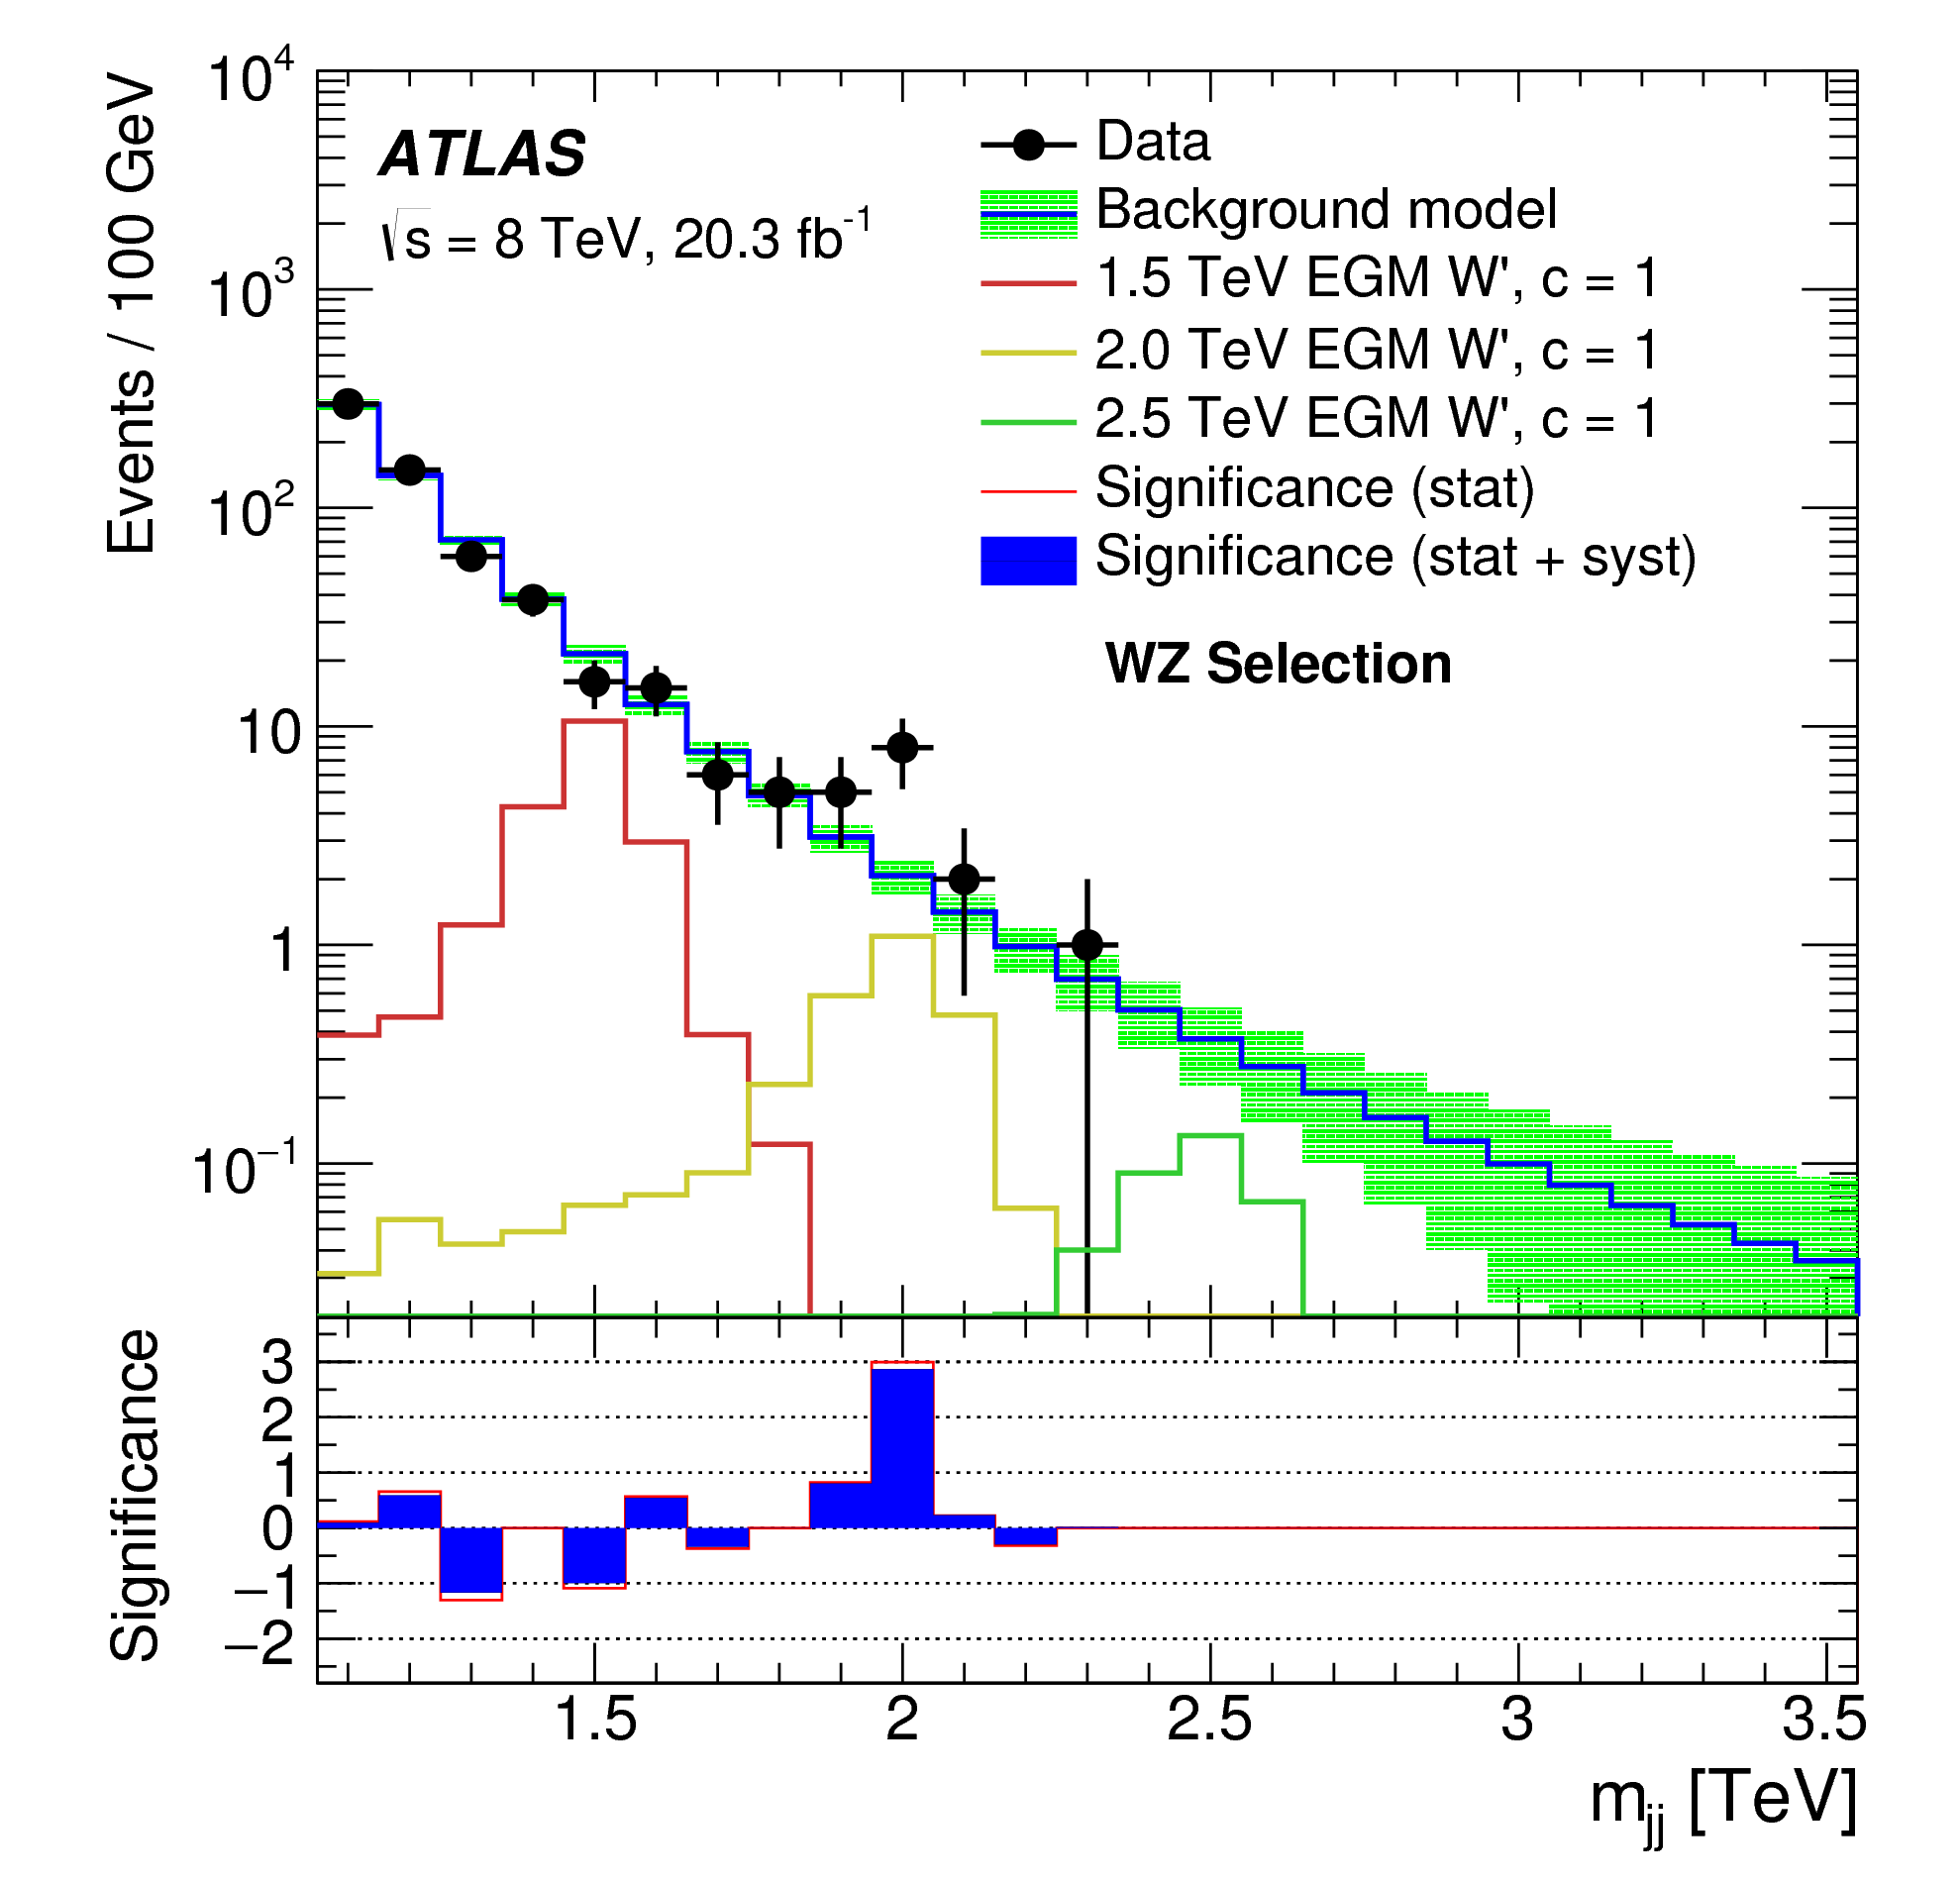
\includegraphics[width=0.4\textwidth]{figures/analysis/search1/misc/atlas_8tev.png}
    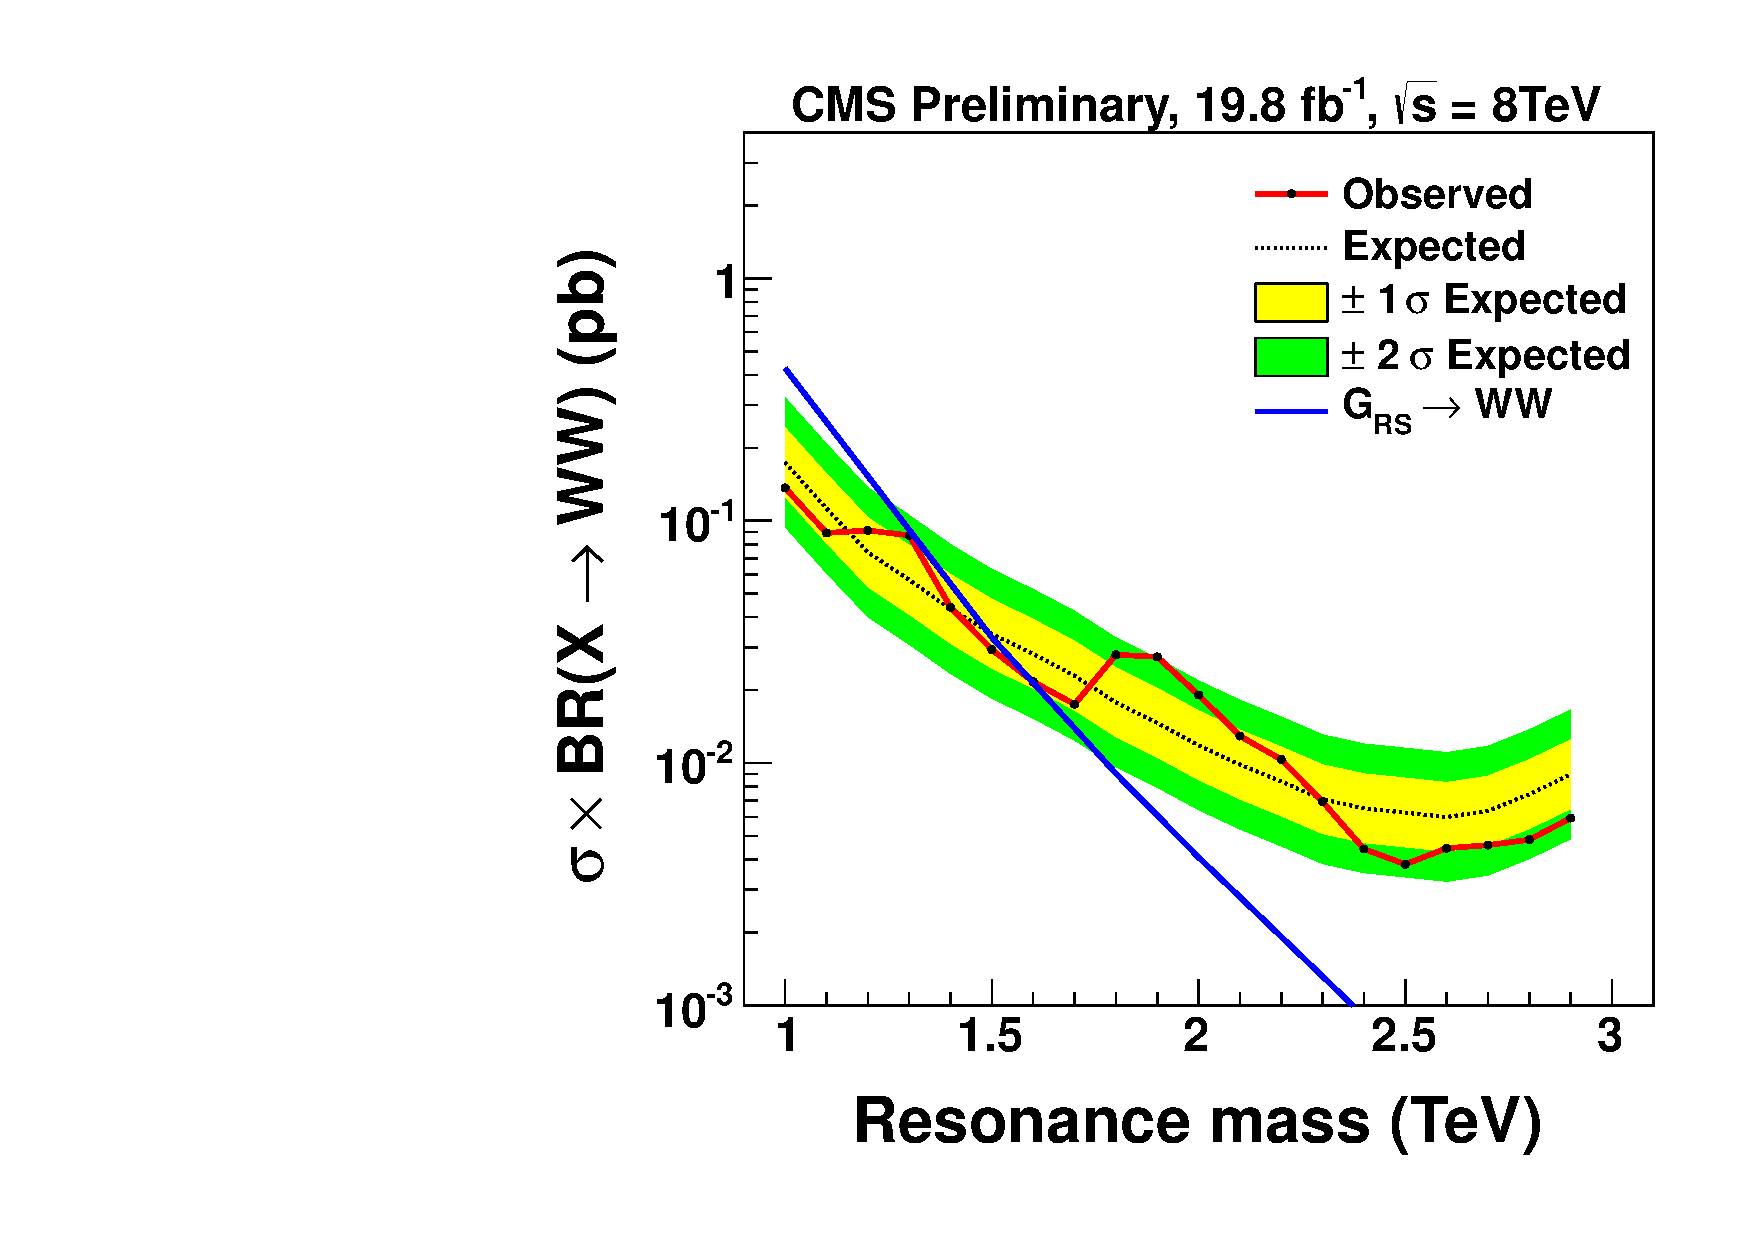
\includegraphics[width=0.4\textwidth]{figures/analysis/search1/misc/EXO-12-024_gWW.pdf}
    \caption{The mass (top) and \PT (bottom) resolution comparing PF only (blue), PF+CHS (red) and PUPPI (pink) jets. The absolute resolution (left) as well as the resolution as a function of the number of reconstructed primary vertices in the event (right)is shown~\cite{Bertolini2014}.}
    \label{fig:searchI:8tev}
\end{figure}

The two measurements were found to be compatible, favoring a heavy resonance with a production cross section of around 5 \fbinv and a mass between 1.9 and 2.0 TeV decaying to either \PW\PW, \PW\PZ or \PZ\PZ~\cite{Dias:2015mhm}. Figure~\ref{fig:searchI:8tevcombo} show the obtained p-value of the ATLAS (red) and CMS (blue) search as well as their combination (black).  

\begin{figure}[ht] 
    \centering
    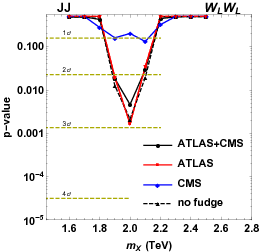
\includegraphics[width=0.25\textwidth]{figures/analysis/search1/misc/CMS_ATLAS_BulkWW_JJ_dijetfit_p.png}
    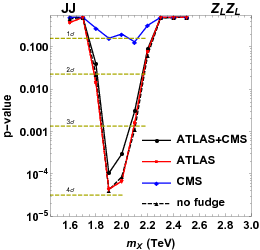
\includegraphics[width=0.25\textwidth]{figures/analysis/search1/misc/CMS_ATLAS_BulkZZ_JJ_dijetfit_p.png}
    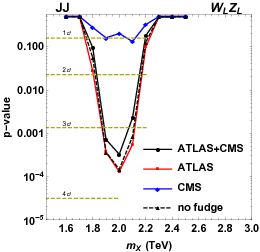
\includegraphics[width=0.25\textwidth]{figures/analysis/search1/misc/CMS_ATLAS_WZ_JJ_dijetfit_p.png}
    \caption{p-values as a function of resonance mass obtained with an emulation of the ATLAS (red) and CMS (blue) searches as well as the combination of the two (black). Here for a \PW\PW (left), \PW\PZ (middle) and \PZ\PZ (right) hypothesis~\cite{Dias:2015mhm}.}
    \label{fig:searchI:8tevcombo}
\end{figure}

The combination of the two excesses and the timing of the ATLAS paper, naturally lead to some excitement and in the coming weeks, the arXiv was flooded with theory papers seeking an explanation for the measurements.
The pressure on seeing early results with 13 TeV data in the VV all-hadronic final state was high, and it was agreed with CMS Physics Coordination that a preliminary analysis would be ready in December that same year, only 6 months after the first 13 TeV collision.

\subsection{Analysis strategy}

When a resonance X with a mass above 1 TeV decays into a vector boson pair, the bosons have a very high energy ($\tilde\PT=\mX/2=500 \GeV$, assuming X is produced at rest). The boson is co-called "boosted". The decay products of a hadronically decaying boosted vector boson, will therefore not appear as back-to-back in the lab frame but rather be very collimated, as described in Section~\ref{sec:objreco:substructure}. This results in a final state with two large high-\PT jets, where an AK R=0.8 jet is expected to fully contain the two quarks coming from the vector boson decay. This is illustrated in Figure~\ref{fig:searchI:merged}.

\begin{figure}[ht] 
    \centering
    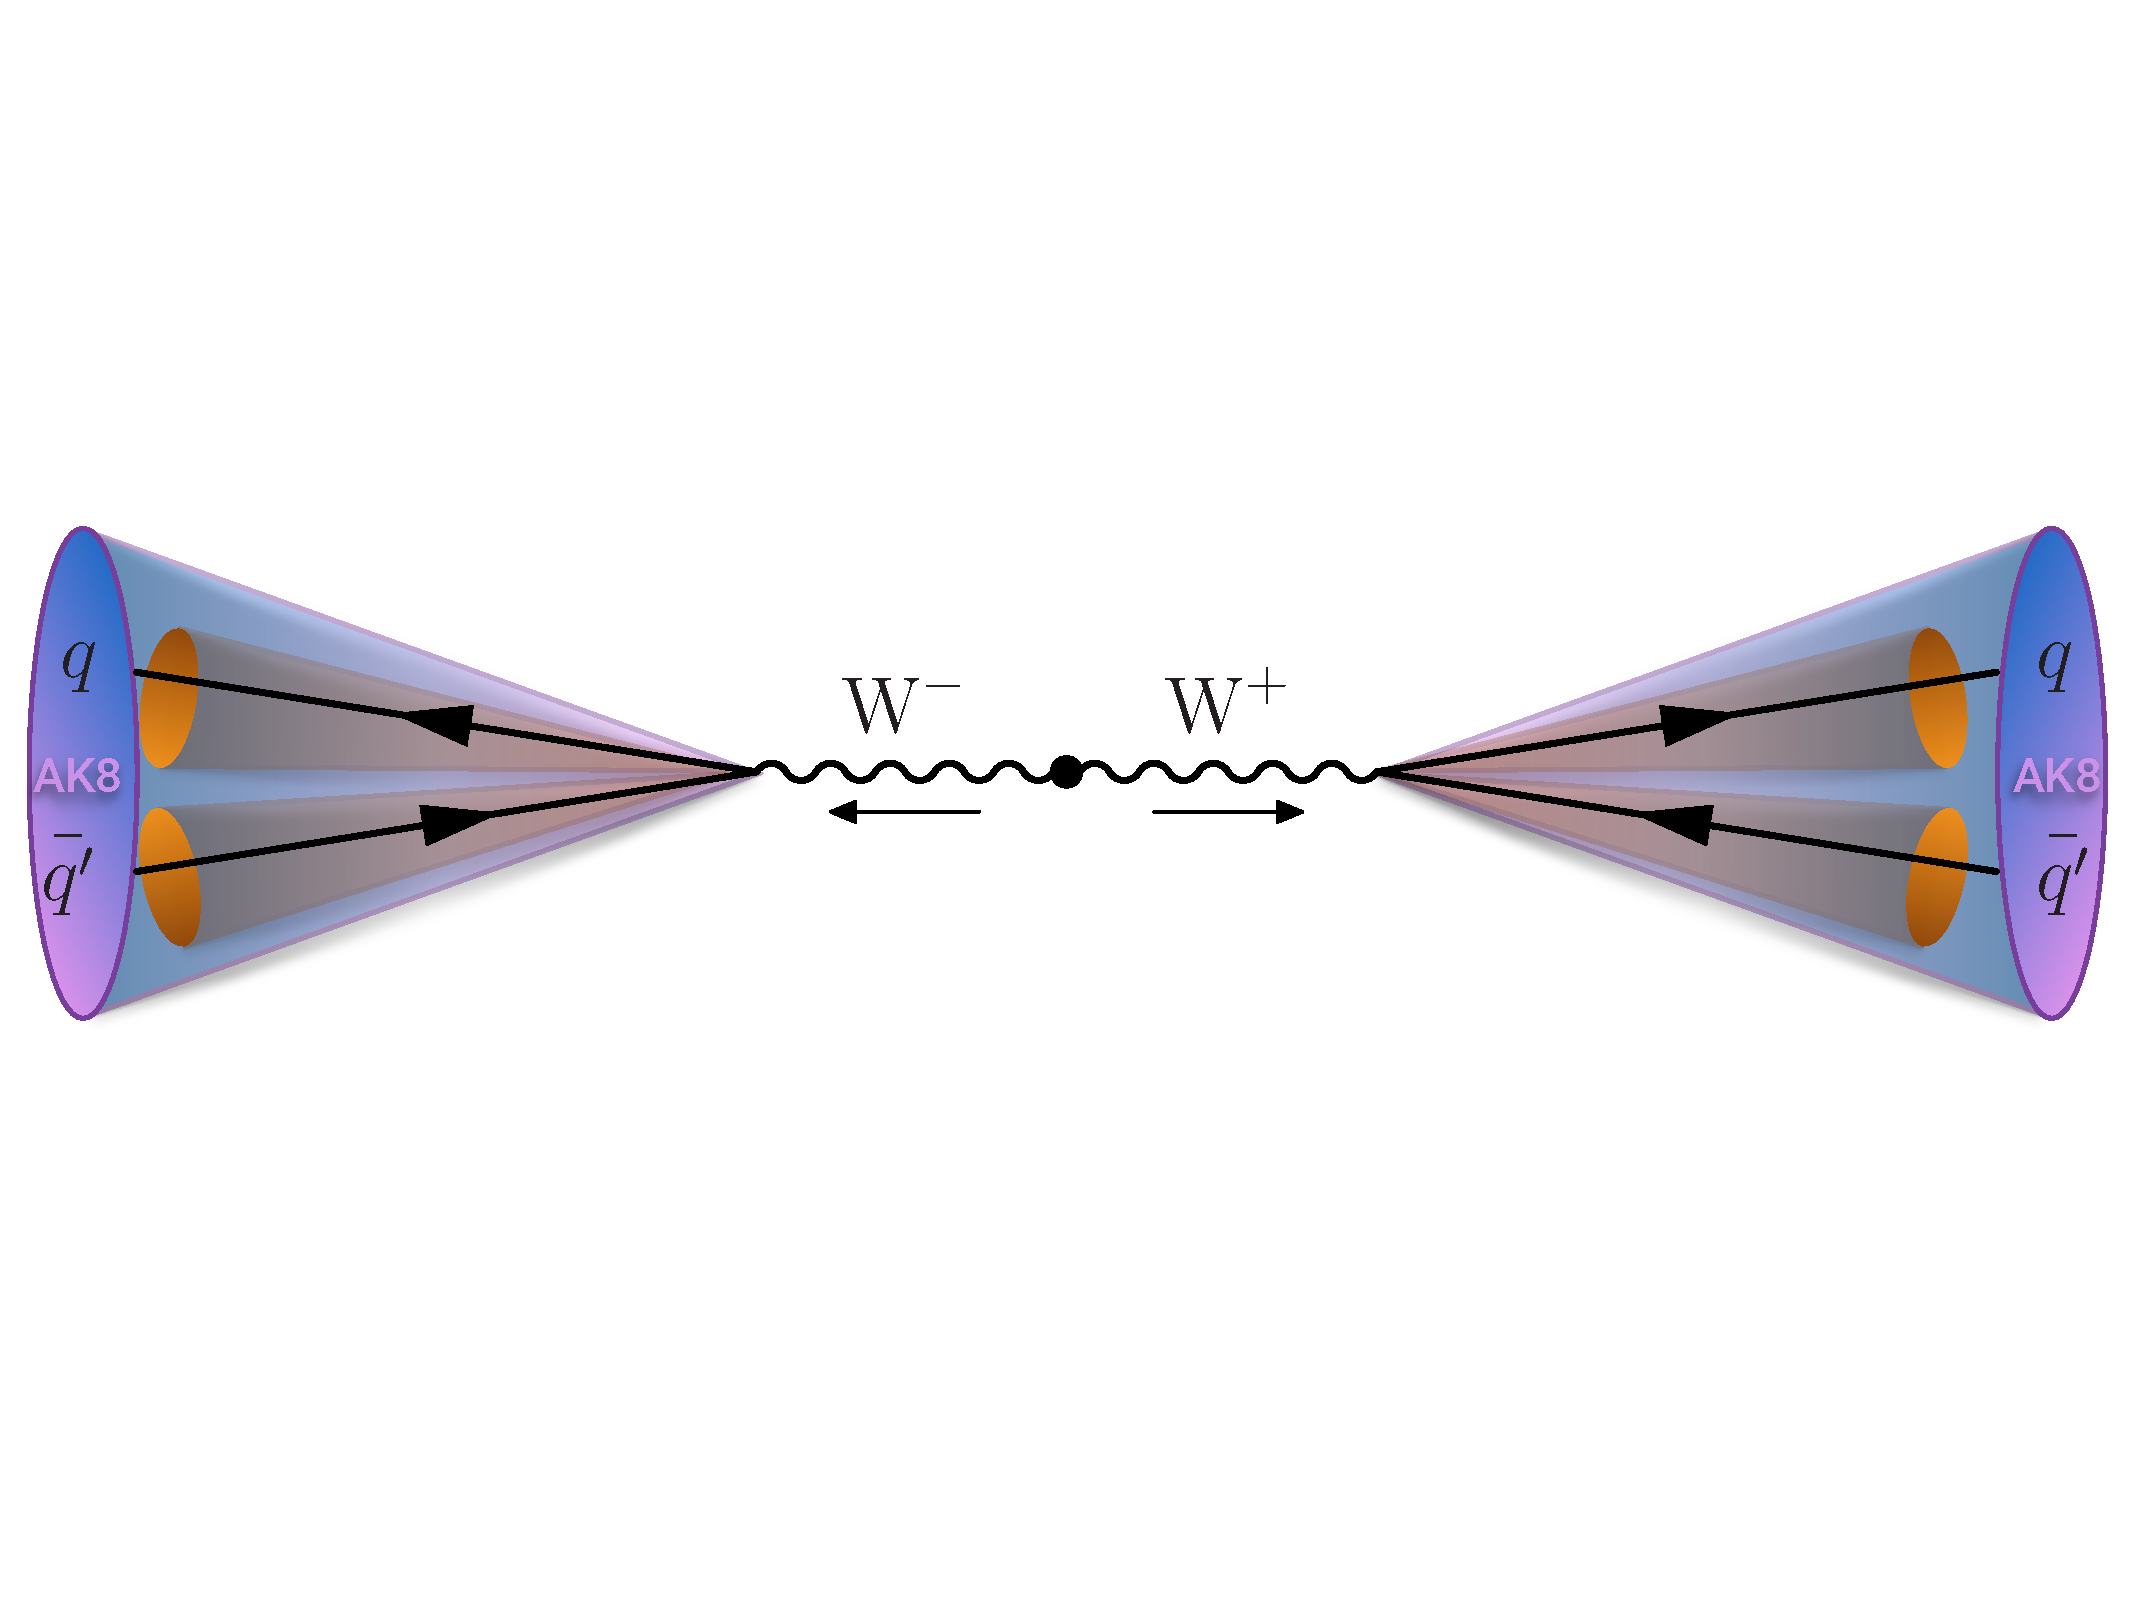
\includegraphics[width=0.70\textwidth]{figures/event_reconstruction/WWqqqq_merged_small.pdf}
    \caption{If a heavy ($>1 \TeV$) resonance decays into vector bosons, the transverse momentum of each boson will be large and its decay products are merged into one single large cone AK8 jet.}
    \label{fig:searchI:merged}
\end{figure}

The two jets are both expected to have a mass around the \PW of \PZ mass, and some intrinsic substructure stemming from their two-prong origin. The invariant mass of the dijet system, \mjj, should be roughly equal to the resonance mass \mX. This dijet system is the final state under scrutiny and the dijet invariant mass is the parameter of interest. Both \WW and \ZZ, as well as \WZ final states are of interest. \par

The main background for such an analysis, is QCD multijet events. As mentioned in Section~\ref{sec:objreco:substructure}, quark/gluon jets can obtain a high mass due to diffuse radiation and QCD processes have such a large cross section that the number of QCD jets with a mass compatible with the W mass can be large. In order to discriminate between the two, we take advantage of three properties: 1. The groomed mass of signal and background jets should be very different, 2. signal jets should appear two-prong like, quark/gluon jets not, and 3. the dijet invariant mass for a signal process should peak around the resonance mass while the QCD spectrum is predicted to be smoothly falling (we will get back to why this assumption is justified in Section~\ref{sec:searchI:bkg}). The strategy therefore consists of performing a smoothness test on \mjj of the observed data, a so-called "bump-hunt", by assuming that the signal will appear as a bump on top of a smooth distribution. This is illustrated in Figure~\ref{fig:searchI:bumphunt}.

\begin{figure}[ht] 
    \centering
    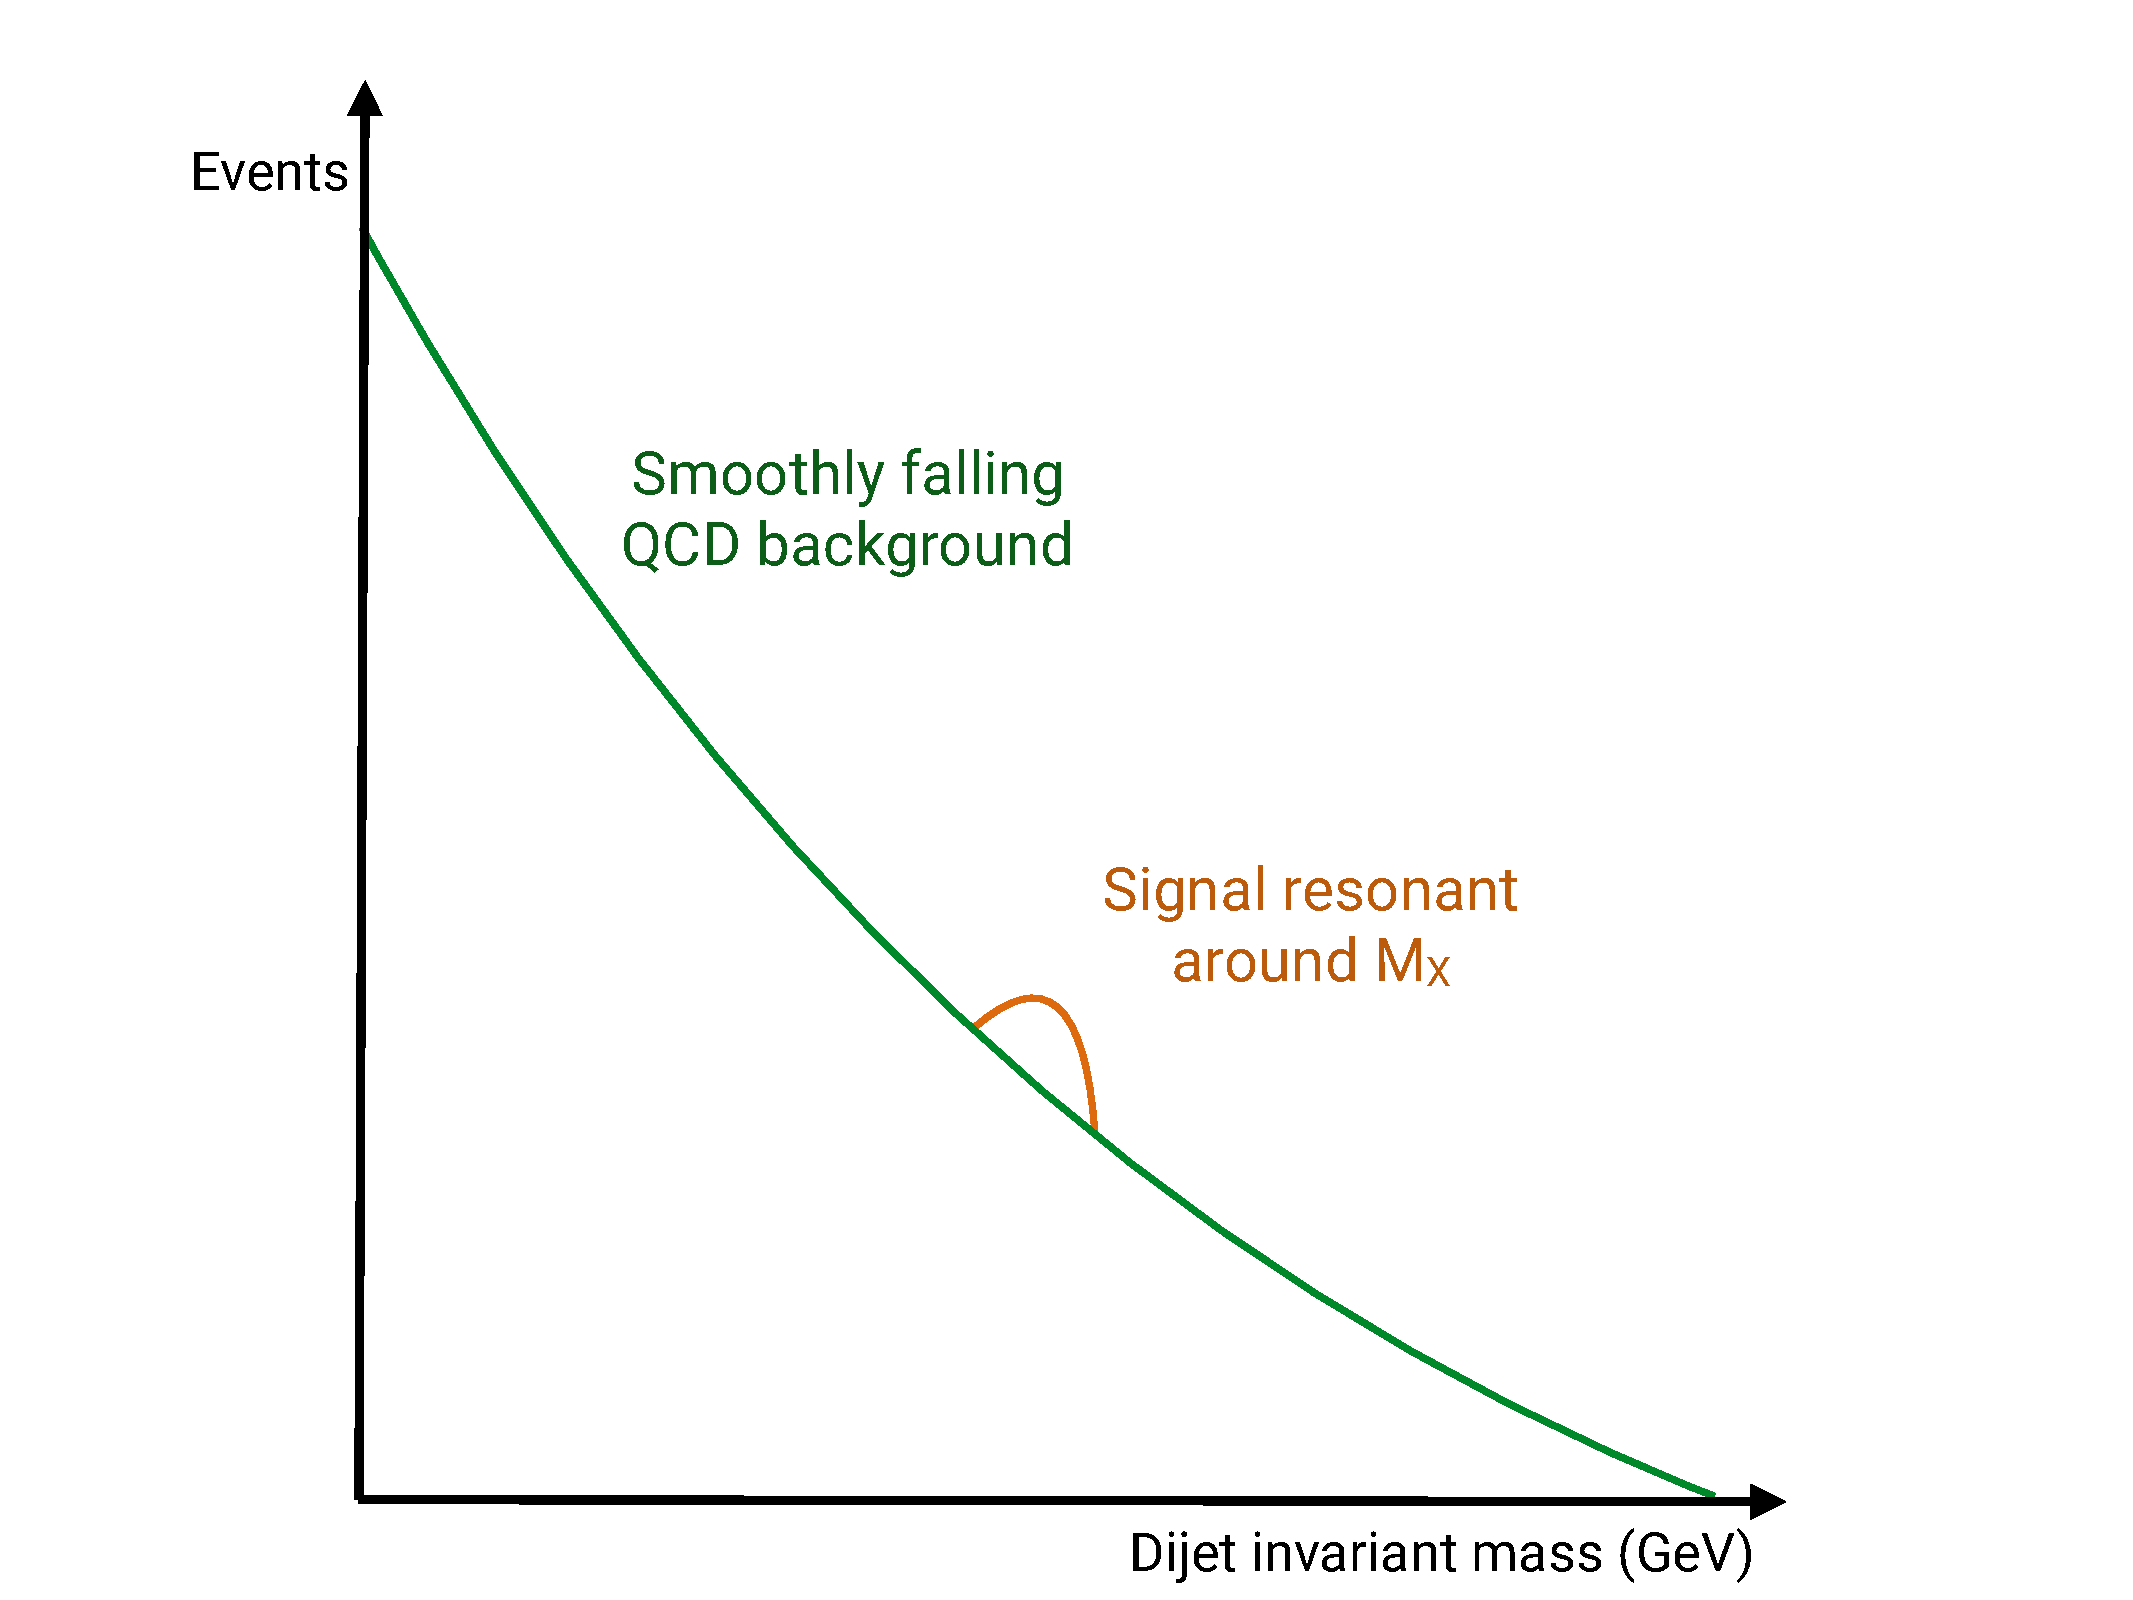
\includegraphics[width=0.50\textwidth]{figures/analysis/search1/misc/sigExtraction.pdf}
    \caption{The search strategy consists of looking for signal "bumps" in the dijet invariant mass on top of a smoothly falling QCD multijet background.}
    \label{fig:searchI:bumphunt}
\end{figure}

The benefit of such a method is that there is no need for any background simulation and the strategy is simple and robust. The disadvantage is that the analysis is intrinsically limited to regions where the dijet invariant mass spectrum is smooth, hence must avoid regions with continuities due to trigger turn-ons or kinematic selections.

\subsection{Data and simulated samples}
The data analyzed in this search correspond to a total integrated luminosity of 2.7\fbinv collected at a center-of mass energy of 13 \TeV between June and December 2015. The instantaneous luminosity of the LHC during this run was around half of the design luminosity ($0.5 \times 10^{34} \percms$), with an average number of primary vertices per event of $<\mu>=13$. \par\par

The bulk graviton model (see Section~\ref{sec:theory:wed}) and the HVT model (\PWpr{} and \PZpr{}, see Section~\ref{sec:theory:hvt}) are used as benchmark signal processes. In these models, the vector gauge bosons are produced with a longitudinal polarization in more than 99\% of the cases, which leads to a 24\% higher acceptance per boson for reasons explained in Section~\ref{sec:objreco:pol}. For the HVT model, a scenario (model B) with $g_{\rm V}=3$, $c_{\rm H}=-0.976243$, and $c_{\rm F}=1.02433$ is chosen, where the heavy resonance predominantly couple to bosons and the coupling to fermions is suppressed. The bulk graviton samples were generated with $\ktilde = 0.5$.
The resonance masses considered lie in the range 1.2 to 4\TeV and has a width of 0.1\% of the resonance mass. The narrow width allows us to neglect detector effect as the natural width of the resonance is smaller than the detector resolution, making the modeling of detector effects on the signal shape independent of the model. All signal samples are generated at leading order with \amcatnlo{} v2.2.2~\cite{Alwall:2014hca} \par\par

Simulated samples of the production of QCD multijet events are generated to leading order using \PYTHIA version 8.205~\cite{Sjostrand:2007gs} with the CUETP8M1 tune~\cite{Khachatryan:2015pea}.


\subsection{Event selection}

\subsubsection{Triggering}
The first selection to be confronted in any analysis, is the trigger selection. Due to an overwhelming QCD background in all-hadronic final states, the threshold for fully-hadronic triggers is very large in order to keep the trigger rate low (preferably around 10-30 Hertz). In this analysis, we therefore decided to take advantage of triggers that place requirements on the jet groomed mass in addition to the "standard" triggers based on the scalar sum of jet transverse energy \HT. These "boosted" triggers were never before tested in data, and this analysis was the first published result taking advantage of grooming at the trigger level in CMS. The following \HT-based triggers (called inclusive triggers in the following) are used
\begin{itemize}
\item \texttt{HLT\_PFHT650\_WideJetMJJ900DEtaJJ1p5}
\item \texttt{HLT\_PFHT650\_WideJetMJJ950DEtaJJ1p5},
\item \texttt{HLT\_PFHT800}
\end{itemize}
where the two first triggers apply an additional cut on the $|\Delta \eta|$ between the two jets for reasons that will be explained below. In addition, two grooming triggers cutting on the jet trimmed mass (see Section~\ref{sec:objreco:trimming}) of 30 and 50 GeV are used
\begin{itemize}
\item \texttt{HLT\_AK8PFJet360\_TrimMass30}
\item \texttt{HLT\_AK8PFHT700\_TrimR0p1PT0p03Mass50}.
\end{itemize}
The tuneable parameters for the trimming algorithm at HLT, were set to $r_{sub}=0.2$ and $p_{T,frac}=0.03$. The \texttt{HLT\_AK8PFJet360\_TrimMass30} trigger is seeded by single-object Level 1 triggers with jet $p_T$ thresholds of 176 or 200 GeV (\texttt{L1\_SingleJet176} or \texttt{L1\_SingleJet200}), and the remaining triggers requires an online \HT{}$>$150 or 175 GeV (\texttt{L1\_HTT150} or \texttt{L1\_HTT175}).\par

In order to avoid any kinks in the dijet invariant mass spectrum due to the presence of a trigger turn-on, we need to define for which dijet invariant mass the analysis triggers are fully efficient ($>99\%$), then cut away everything below that point.

In order to estimate the trigger efficiency, we use a lower threshold prescaled \HT{} trigger \texttt{HLT\_PFHT650} as reference trigger. This trigger has a prescale of 40, meaning it only stores information for every 40 events that trigger it, and is seeded by L1 triggers \texttt{L1\_HTT150} or \texttt{L1\_HTT175}. We then define the efficiency as
\begin{equation*}
\textrm{Efficiency} = \frac{N_{trigger+ref}}{N_{ref}}  
\end{equation*}
where $N_{trigger+ref}$ corresponds to events passing the trigger under study as well as the reference trigger and $N_{ref}$ corresponds to all events passing the reference trigger. Figure~\ref{fig:searchI:trigger-fits} shows the trigger turn-on curves as a function of dijet invariant mass for jets where one of the jets is required to have a pruned mass larger than 65 GeV (in other words, compatible with a W jet). A sharp turn-on for the inclusive triggers (top left) is observed, reaching the 100\% efficiency plateau for dijet masses of around 1.0--1.1 TeV. The grooming triggers, however, turn on more slowly and are not fully efficient before dijet invariant masses of around 1.2 TeV (top right). The real power of the grooming triggers become clear when adding them in OR with the \HT-based triggers. The bottom plot in Figure~\ref{fig:searchI:trigger-fits} compares the trigger turn-on curves as a function of dijet invariant mass for jets passing one of the three inclusive triggers only, one of the grooming triggers only and when combining all of them. Here, one can see that the 99\% efficiency threshold is lowered by 75 \GeV when including the substructure triggers, once substructure is required at analysis level.
This allowed for the analysis to start at a dijet invariant mass of 1 TeV.

\begin{figure}[h!]
\centering
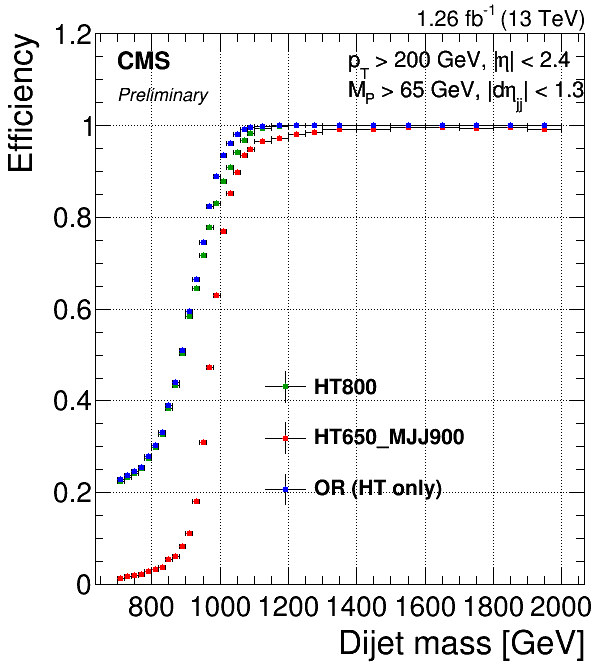
\includegraphics[width=0.4\textwidth]{figures/analysis/search1/AN-15-211//triggereffMjj-HT.png}
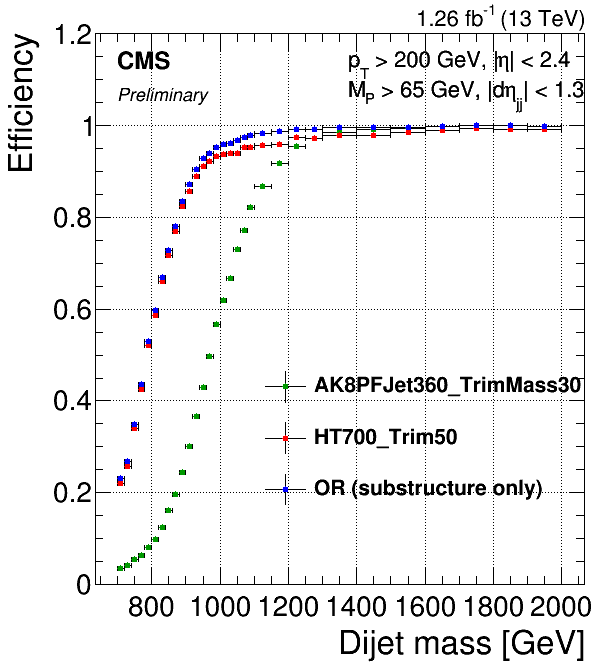
\includegraphics[width=0.4\textwidth]{figures/analysis/search1/AN-15-211//triggereffMjj-SUBST.png}\\
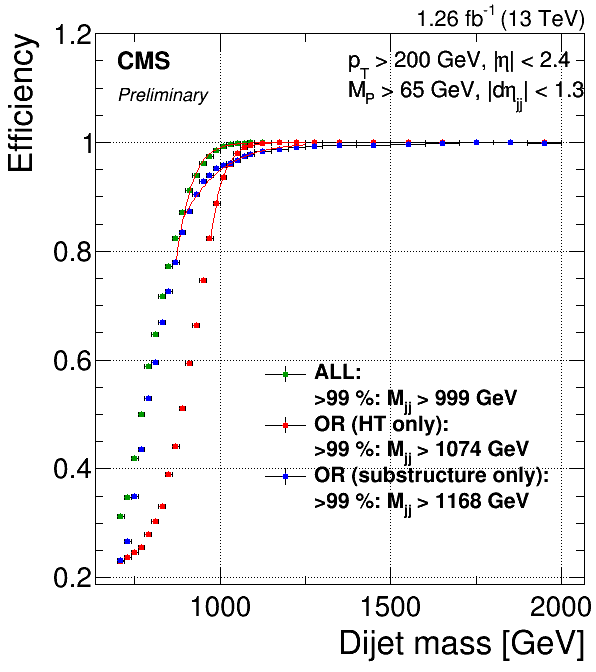
\includegraphics[width=0.4\textwidth]{figures/analysis/search1/AN-15-211/triggereffMjj-ALL.png}
\caption{Top: Efficiency for the inclusive triggers (top left) and the grooming triggers (top right) as a function of dijet invariant mass for jet pairs where one jet has a pruned mass larger than 65 GeV. Bottom: Comparison of trigger efficiencies for jets passing one of the HT-triggers only (red), for jets passing one of the grooming-triggers only (blue) and for jets passing one of the HT-triggers or one of the grooming triggers (green). Here as a function of dijet invariant mass for all jet pairs passing loose selections and where one jet has a pruned mass larger than 65 GeV. The 99\% efficiency threshold is lowered by 75 \GeV when including substructure taggers.}
\label{fig:searchI:trigger-fits}
\end{figure}


As a measure of the performance of the grooming triggers, we have in addition looked at the trigger efficiencies as a function of the offline groomed mass (pruned and softdrop, see Sections~\ref{sec:objreco:pruning} and ~\ref{sec:objreco:softdrop}), for the grooming trigger with the lowest mass threshold (30 \GeV). This is shown in Figure~\ref{fig:searchI:grooming-mj-trigger}, where an additional cut on the jet transverse momentum of one of the jets of 600 GeV is required and no other mass cut is applied. The trigger plateau is reached for offline groomed-jet masses around 50 GeV, an impressively sharp turn-on for a trigger paths first test i data (as reference trigger for this study, the prescaled trigger \texttt{HLT\_PFJet320} was used). 

\begin{figure}[h!]
\centering
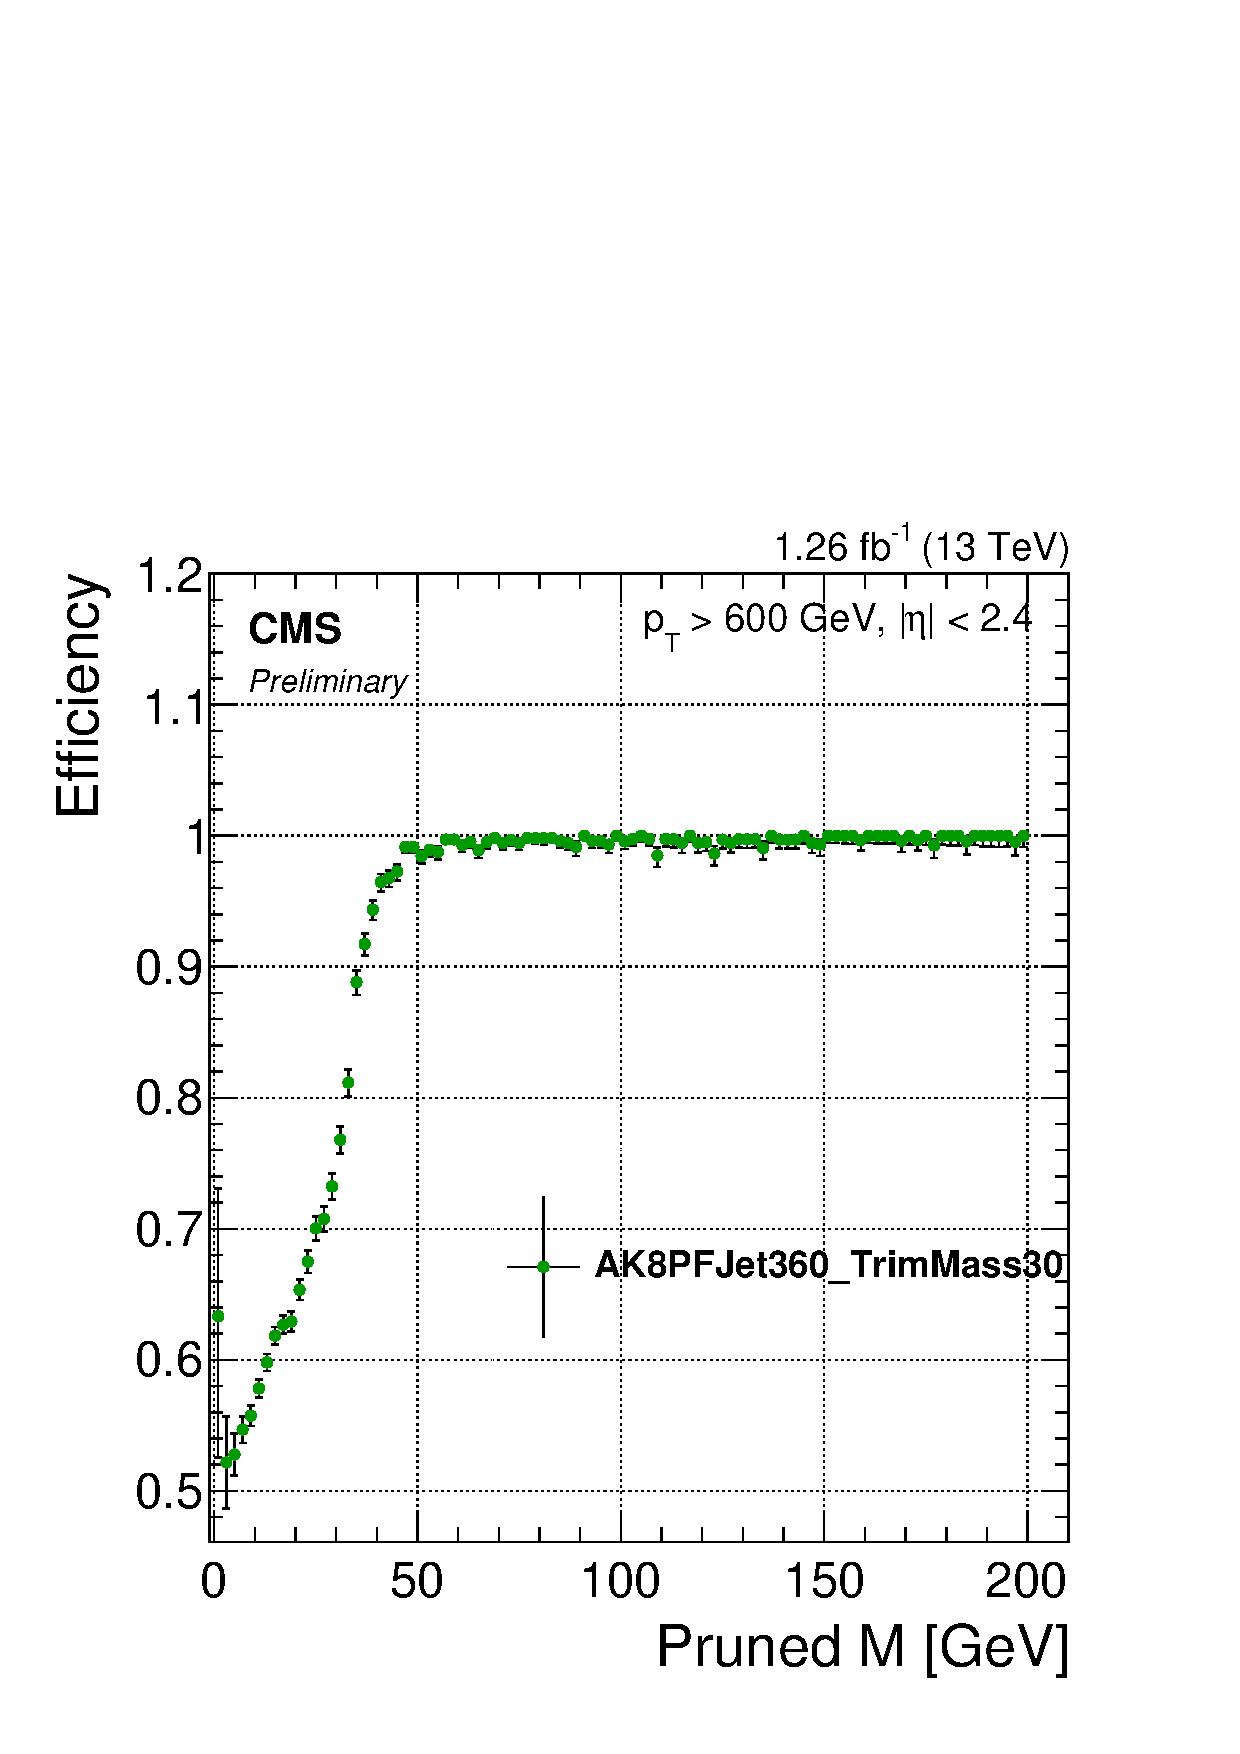
\includegraphics[width=0.4\textwidth]{figures/analysis/search1/AN-15-211//triggereff-prunedmass600.pdf}
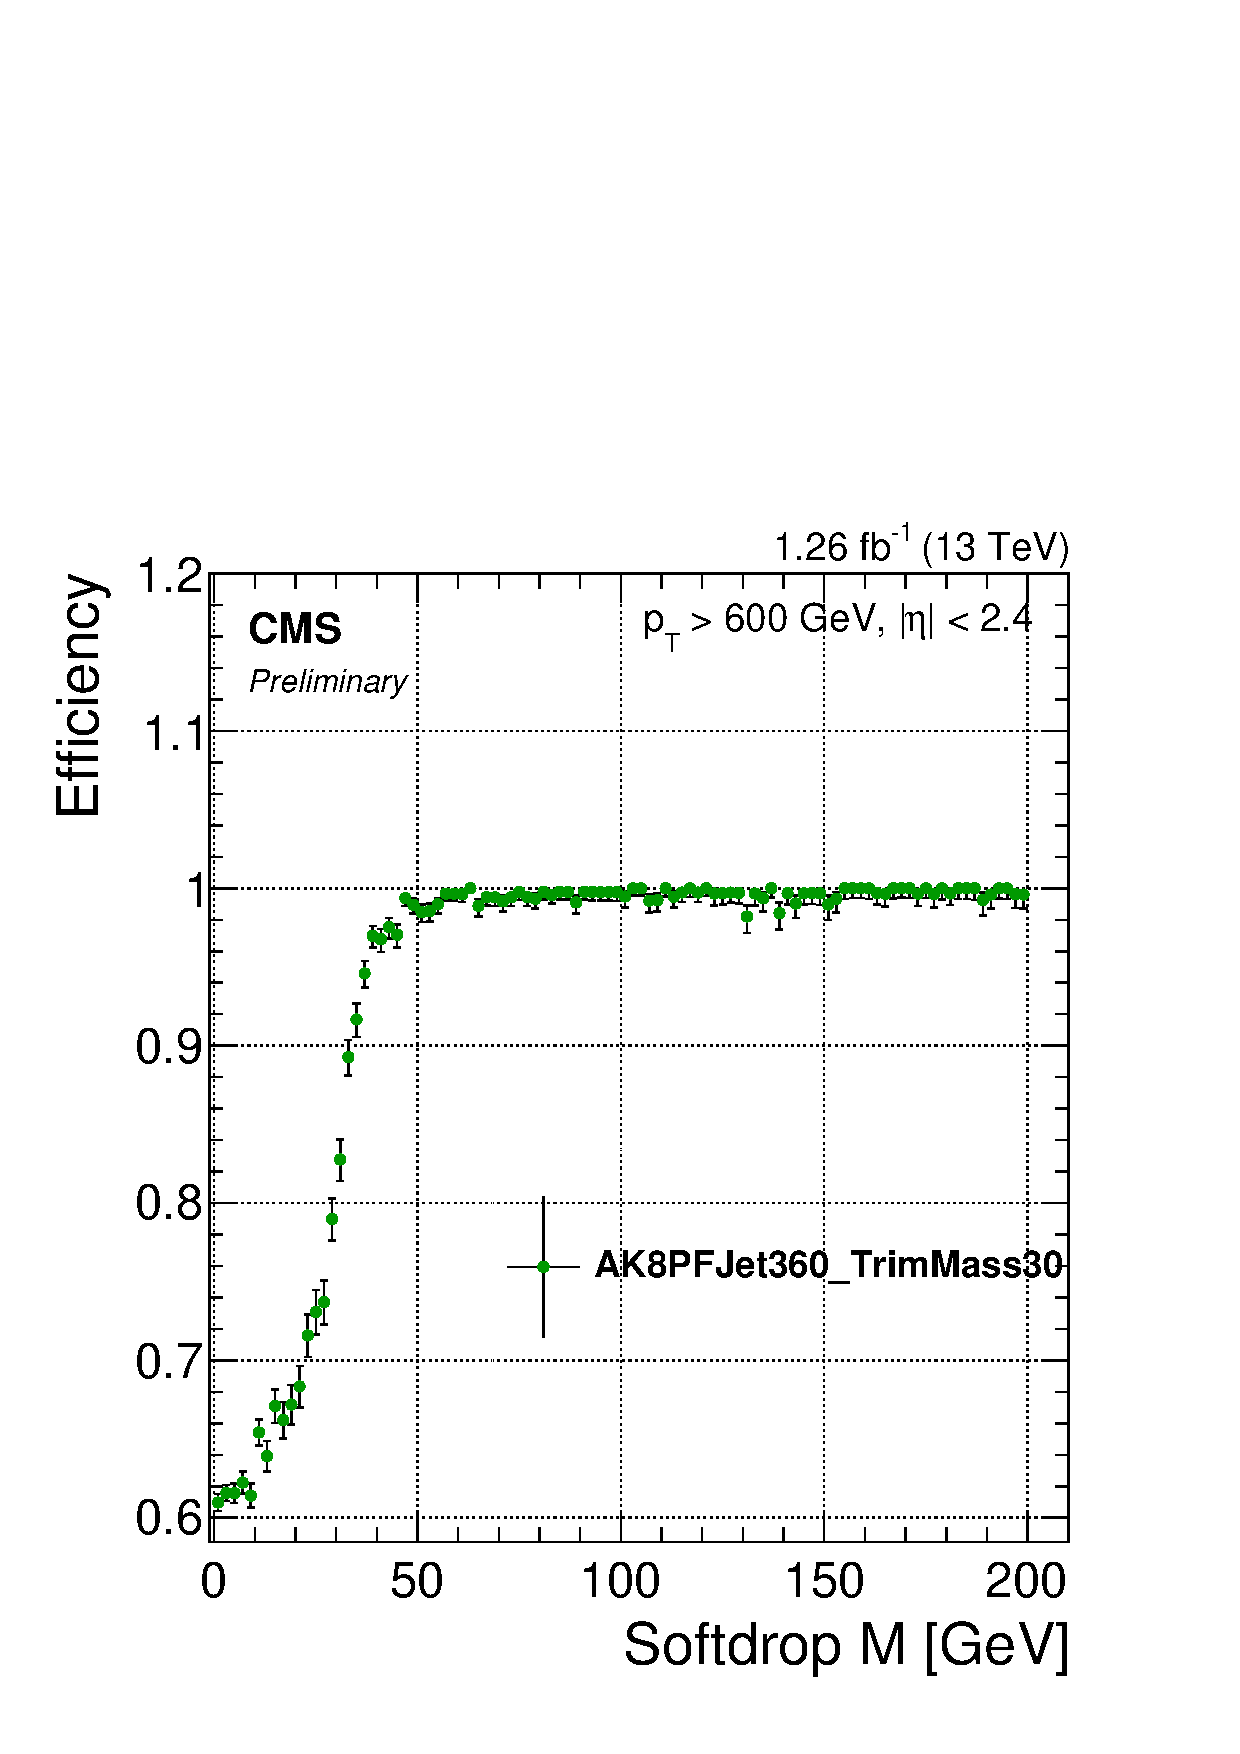
\includegraphics[width=0.4\textwidth]{figures/analysis/search1/AN-15-211//triggereff-sdmass.pdf}
\caption{Efficiency for the lowest threshold grooming trigger as a function of pruned-jet (left) and softdrop-jet (right) mass for jets with $\PT > \unit{600}{\GeV}$.}
\label{fig:searchI:grooming-mj-trigger}
\end{figure}


\subsubsection{Preselection} 
After trigger selections and the corresponding requirement of a dijet invariant mass above 1 \TeV to ensure a smoothy falling background, the process of maximizing the signal significance while keeping the background low can begin. This is done through a set of jet requirements. The jets used in this analysis are clustered with the anti-\kt{} jet clustering algorithm with a clustering parameter of $R=0.8$ (see Section ~\ref{sec:objreco:jets}) to allow containment of the full vector boson decay products. These jets are further required to pass certain jet identification requirements provided by the JetMET POG~\cite{jetID_JME}, in order to distinguish them from fake jets. These are as follows:
\begin{itemize}
\item Number of Constituents $> 1$, for all jet $\eta$
\item Neutral Hadron Energy Fraction $< 0.90$, for all jet $\eta$
\item Neutral EM Energy Fraction $< 0.90$, for all jet $\eta$
\item Charged Hadron Multiplicity $> 0$, for jet $|\eta| < 3.0$
\item Charged EM Energy Fraction $< 0.99$, for jet $|\eta| < 3.0$
\end{itemize} 
Jets are further corrected for nonlinearities in $\PT$ and rapidity using standard jet energy corrections at CMS as described in Ref.~\cite{jme_jinst} for $R$=0.8 anti-\kt{} jets.
As we know that a minimum transverse of 200 \GeV is required for the decay products of a \PW/\PZ to be fully contained within an R=0.8 jet, events are further selected by requiring at least two jets with $\PT > \unit{200}{\GeV}$. These are in addition required to be central, with an $|\eta| < 2.4$. \par
The two highest \PT jets in the event passing these criteria are selected as potential vector boson candidates.
As our main background is QCD multijet events, we further take advantage of the fact that the angular distribution between these, mainly t-channel, processes are very different from the s-channel signal processes under study. The crossection for QCD t-channel processes as a function of the opening angle with respect to the beam axis ($\theta*$), exhibit a pole around $\cos \theta*=1$, meaning QCD t-channel jets are mostly forwardly produced, with an opening angle with respect to the beam axis close to zero. The signal jets on the other hand, produced through an s-channel process, are concentrated in the barrel region. We therefore require the jets to have a separation of $|\Delta\eta|<1.3$ in order to reduce the QCD multijets background.
The distribution of $|\Delta\eta|$ between the two highest-\PT jets for QCD as well as for different signal scenarios, is shown in Figure~\ref{fig:searchI:detaopt}

\begin{figure}[h!]
\centering
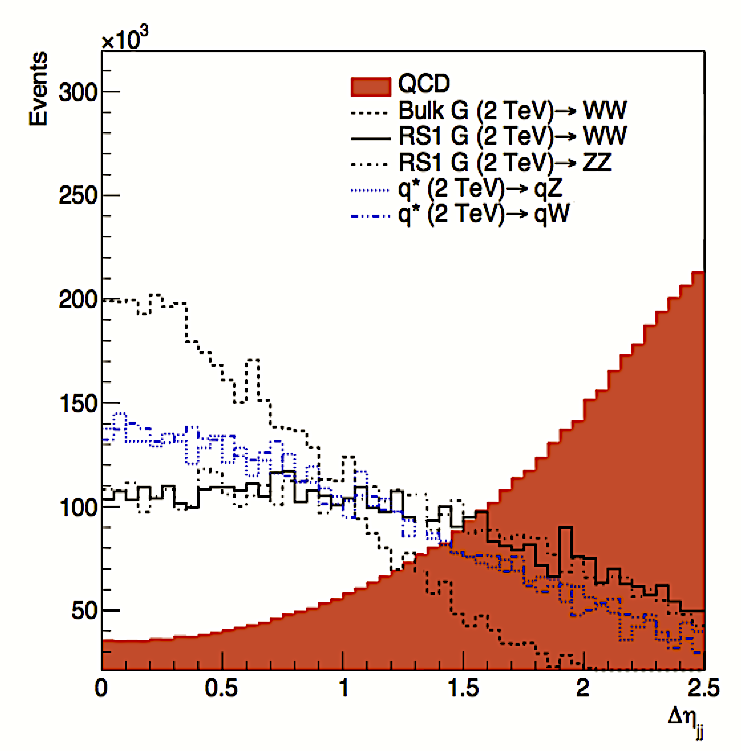
\includegraphics[width=0.4\textwidth]{figures/analysis/search1/misc/deta_opt.png}
\caption{ $|\Delta\eta|$  between the two highest-\PT jets for QCD jets and jets stemming from different signal scenarios.}
\label{fig:searchI:detaopt}
\end{figure}
 
A cut of $|\Delta \eta|_{jj}<1.3$ makes sure to remove the t-channel pole at $\cos \theta* = 1$ and is in addition found to yield the best separation between signal and the QCD background

A summary of the applied preselections is as follows:

\begin{itemize}
\item PF jet tight ID applied
\item Jet $\eta < 2.4$
\item Jet \pt $> 200$ GeV
\item $|\Delta\eta|_{jj} < 1.3$
\item Dijet invariant mass $> 1$ TeV
\end{itemize} 

The \PT, $\eta$, dijet invariant mass and $|\Delta \eta|_{jj}$ distribution for the two leading jets in the event after the above preselections have been applied is shown in Figure~\ref{fig:kinematics-all}.

\begin{figure}[h!]
\centering
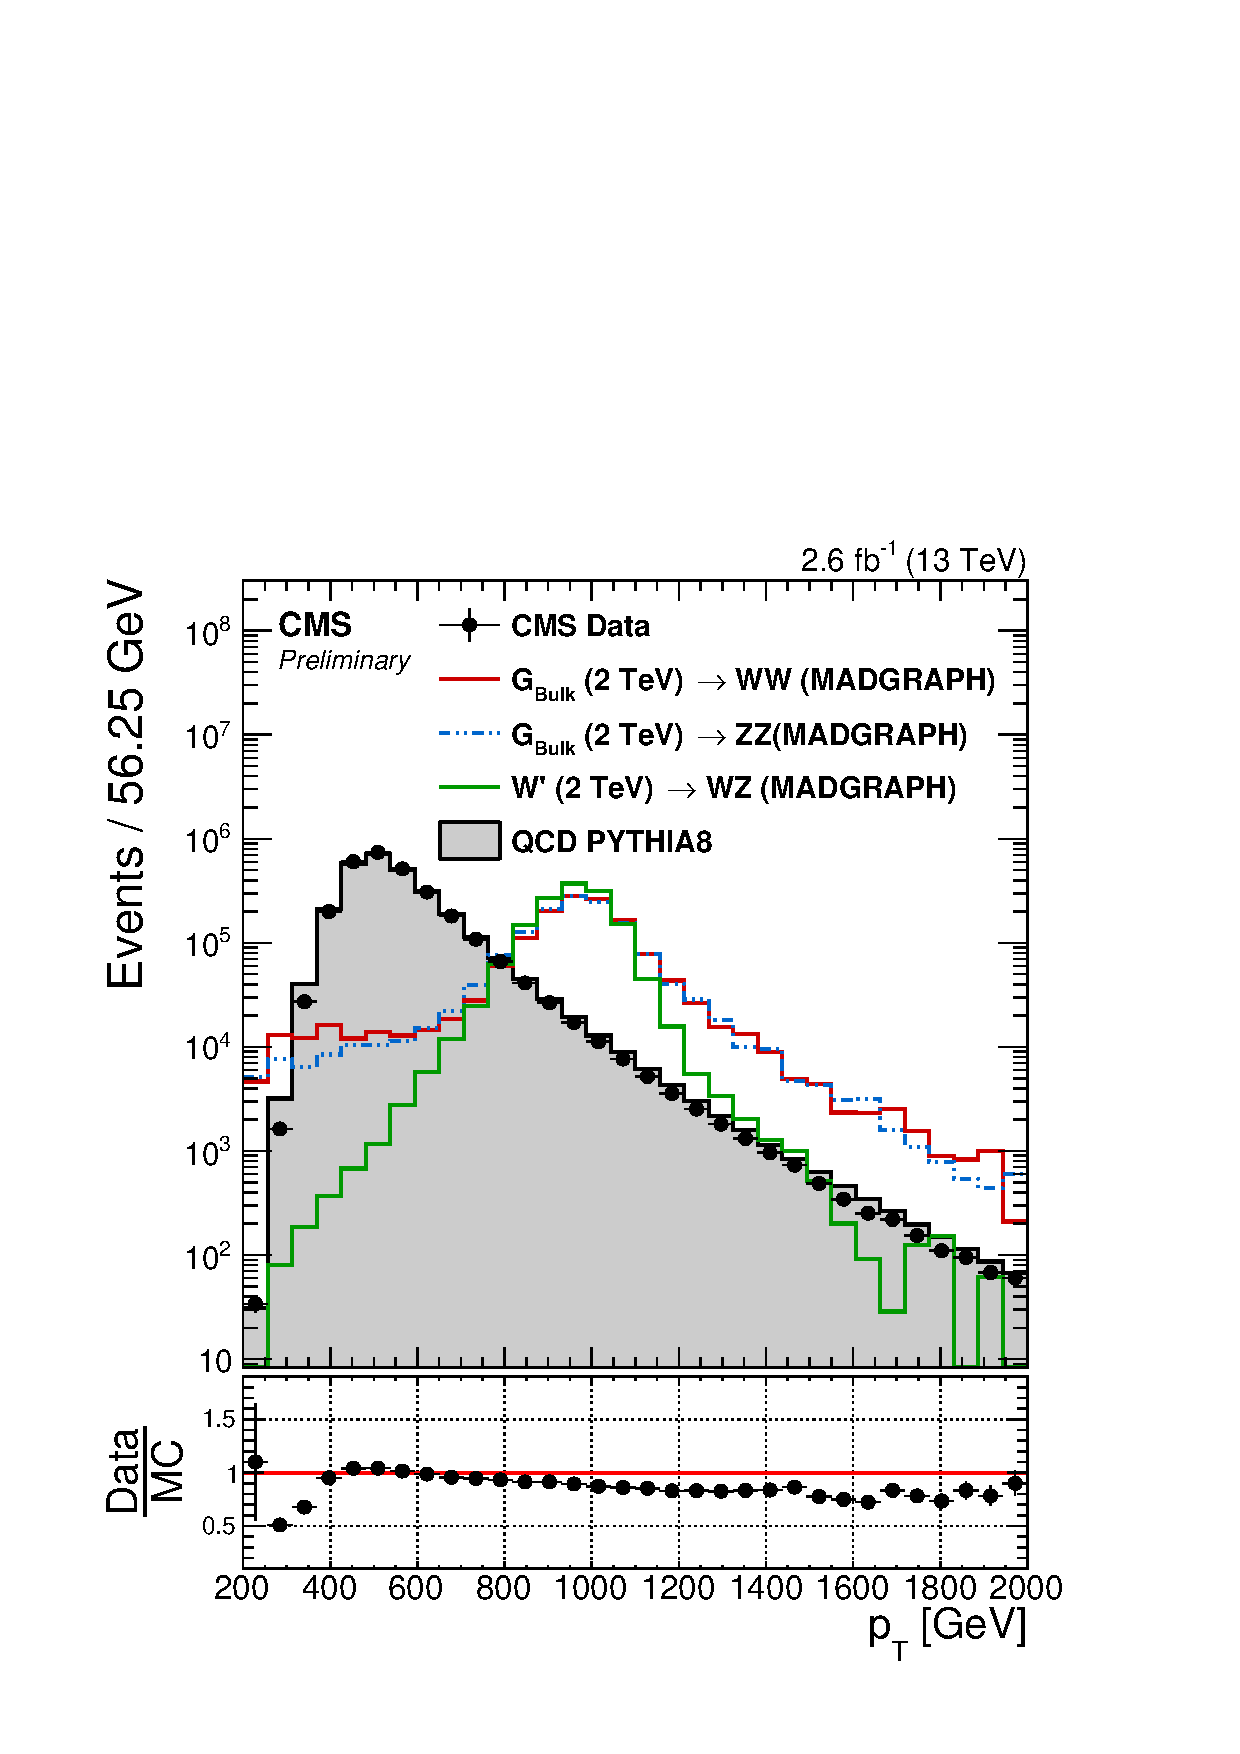
\includegraphics[width=0.4\textwidth]{figures/analysis/search1/AN-15-211/controlplots/silverjson/Pt_WSignal.pdf}
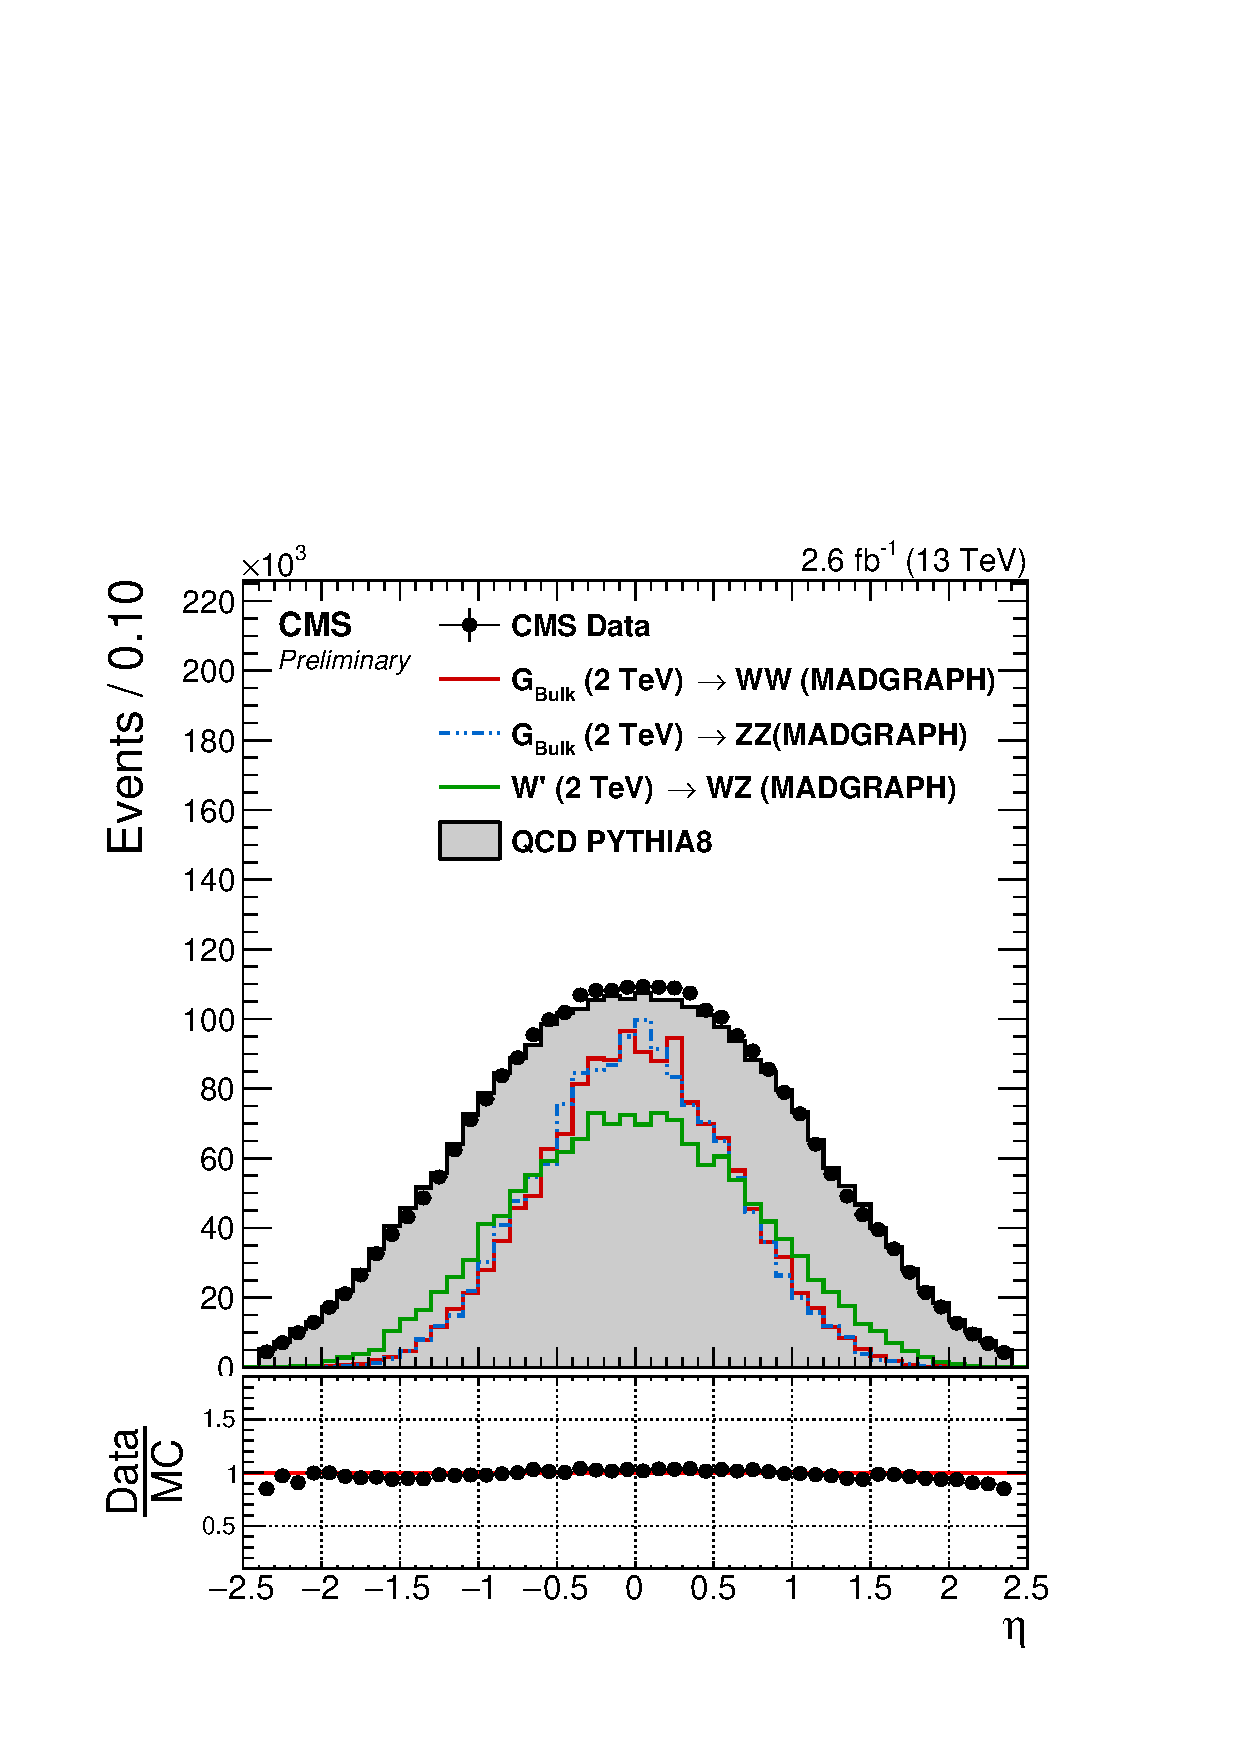
\includegraphics[width=0.4\textwidth]{figures/analysis/search1/AN-15-211/controlplots/silverjson/Eta_WSignal.pdf}\\
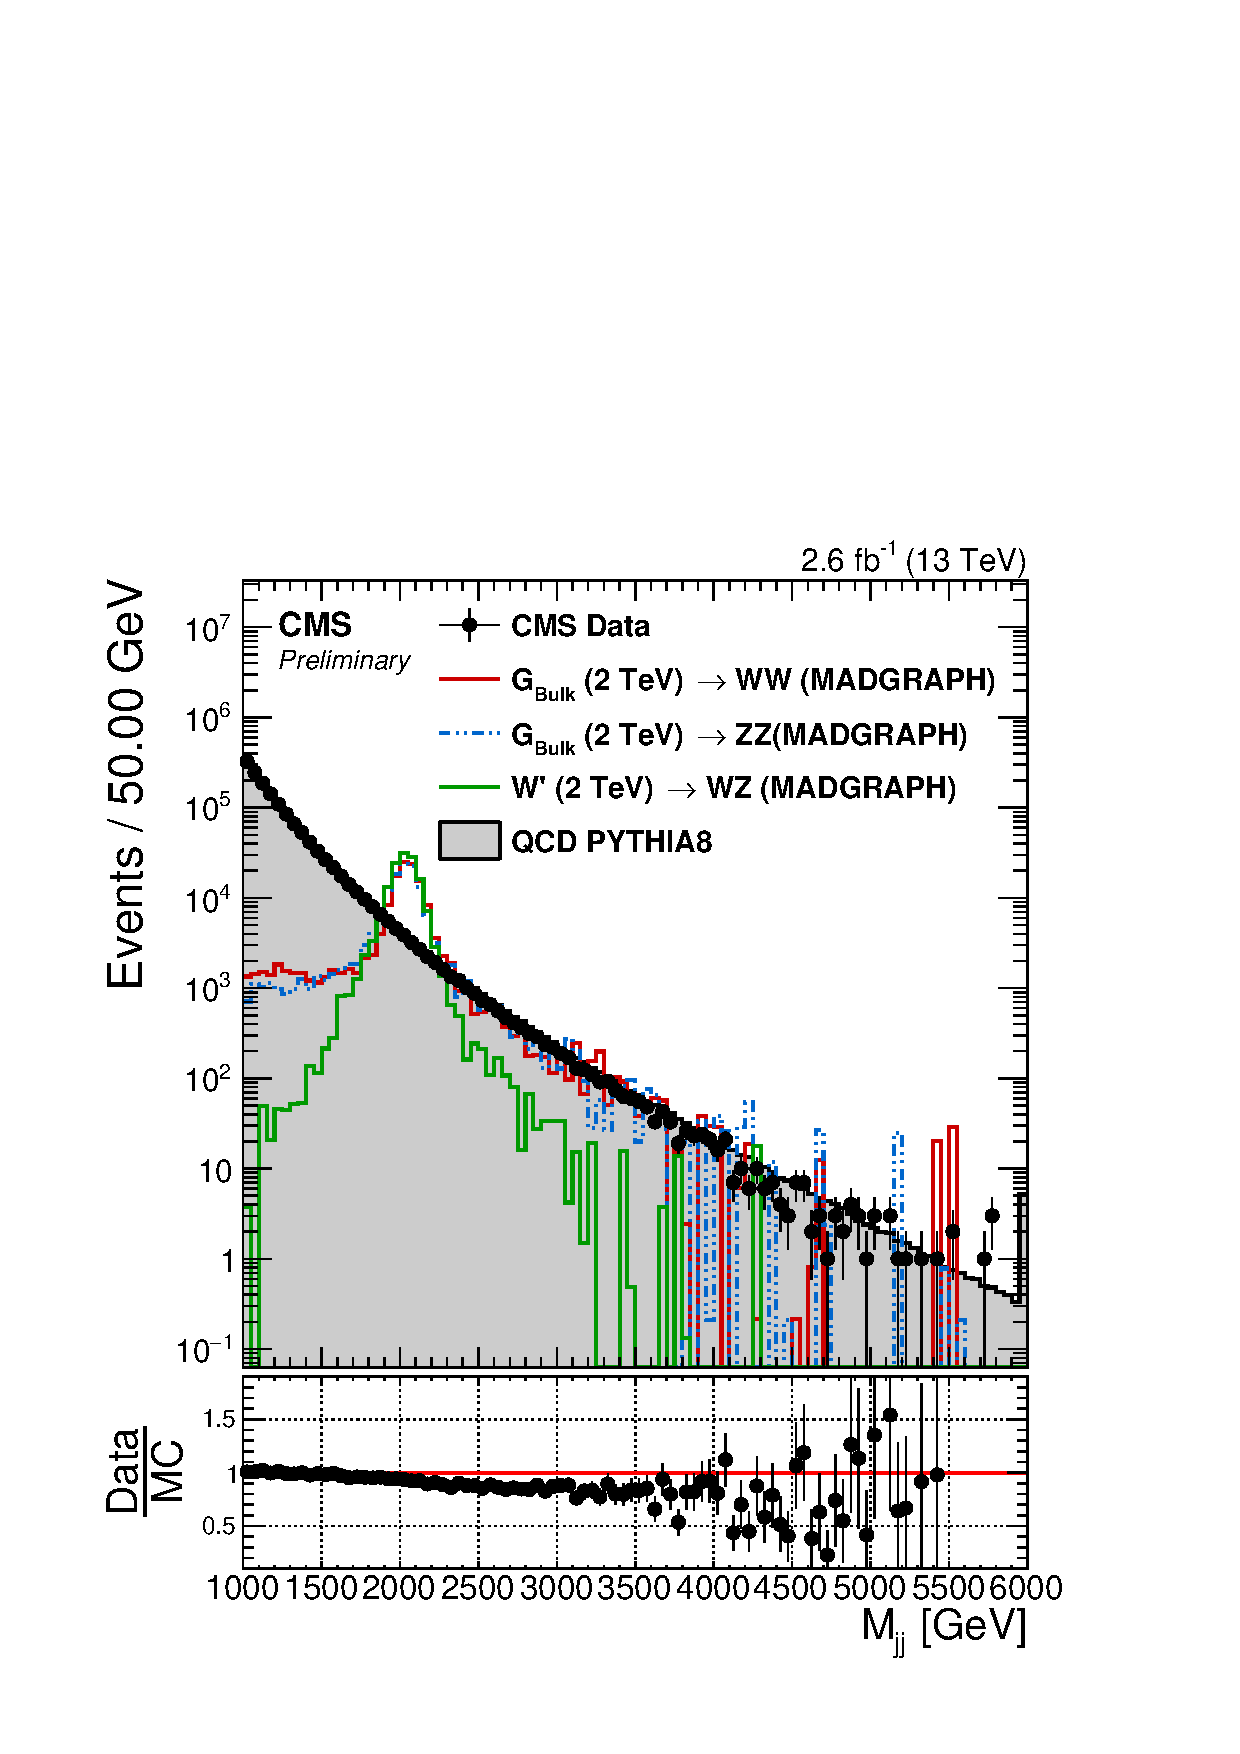
\includegraphics[width=0.4\textwidth]{figures/analysis/search1/AN-15-211/controlplots/silverjson/Mjj_WSignal.pdf}
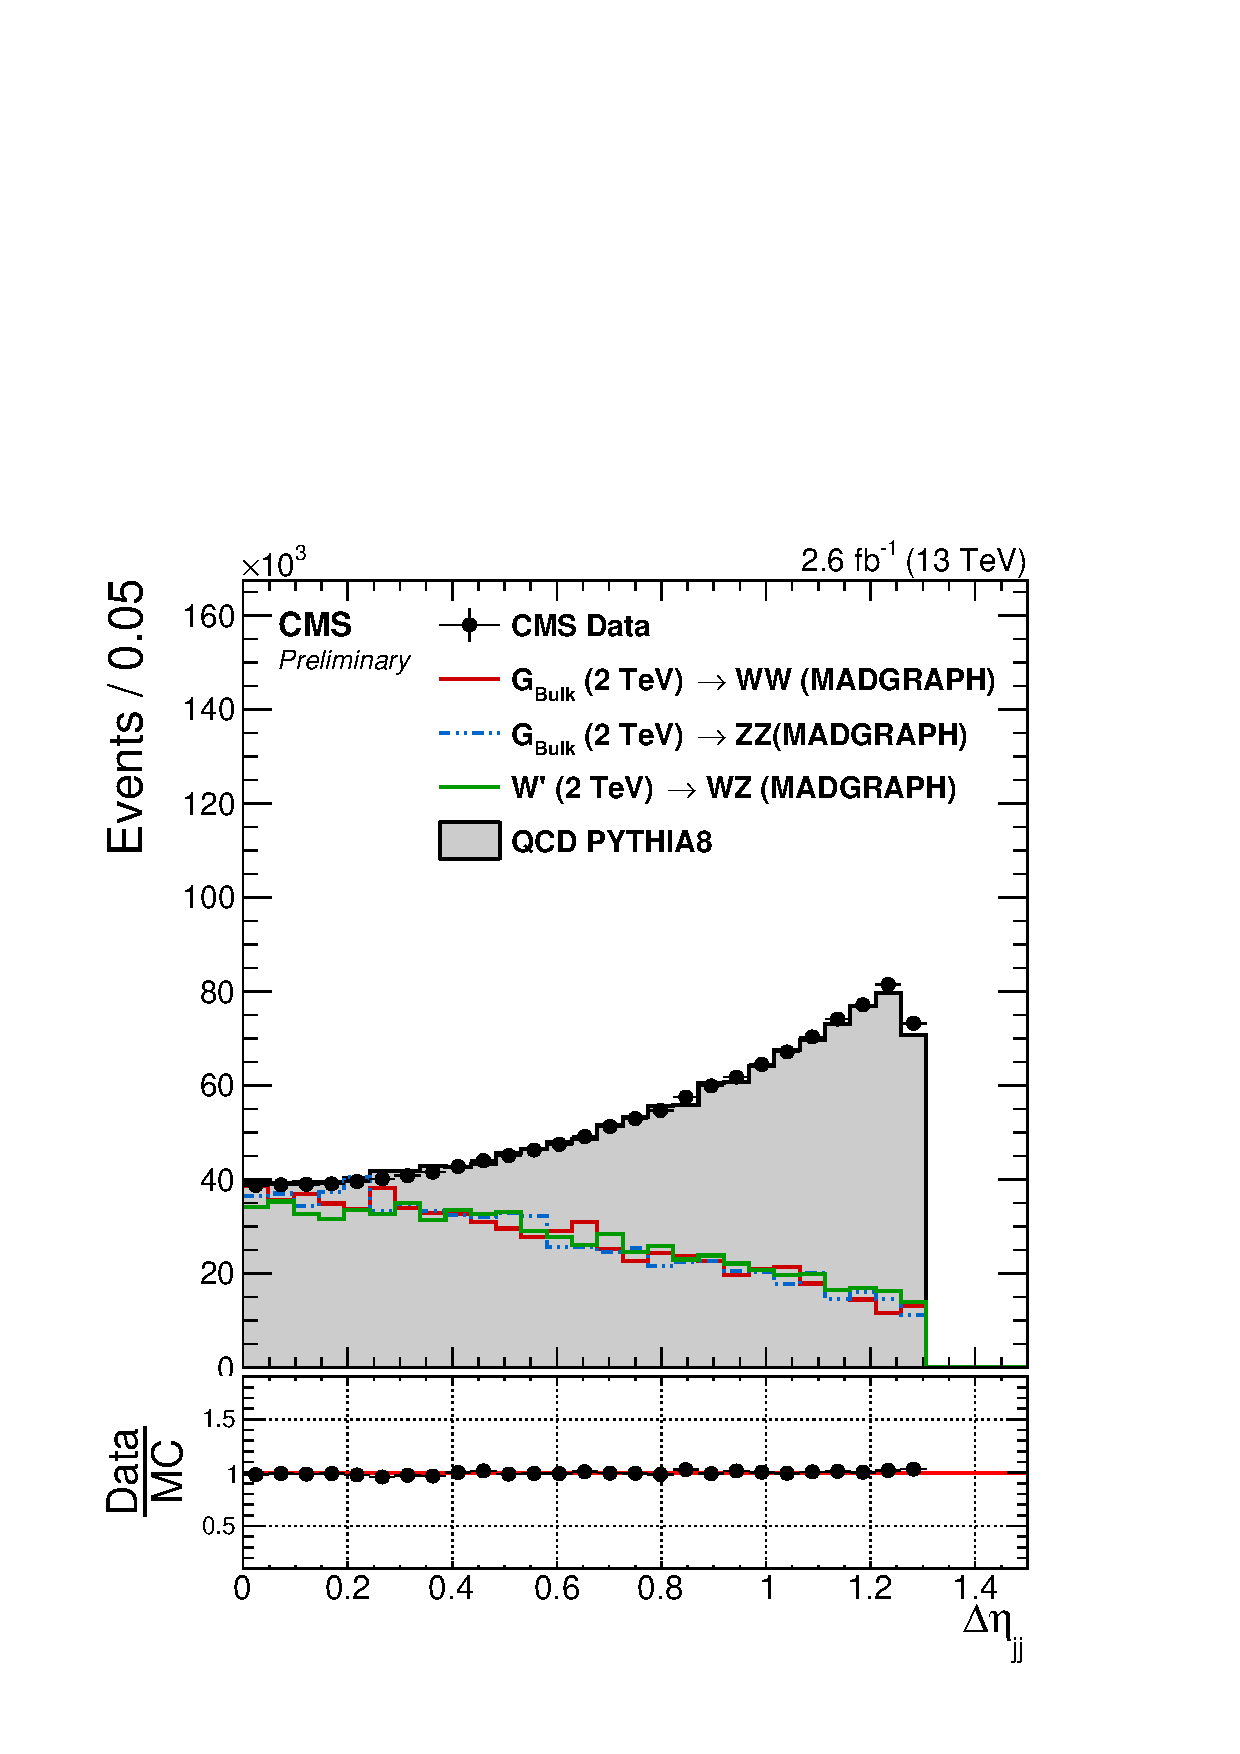
\includegraphics[width=0.4\textwidth]{figures/analysis/search1/AN-15-211/controlplots/silverjson/DeltaEta_WSignal.pdf}
\caption{Jet \PT (top left), $\eta$ (top right), dijet invariant mass (bottom left) and $|\Delta \eta|_{jj}$ (bottom right) distribution for the two leading jets in the event after loose preselections are applied. The signal is scaled by an arbitrary number.}
\label{fig:kinematics-all}
\end{figure}

\subsubsection{Vector boson tagging}

After preselections, we take advantage of the jet substructure algorithms described in Section~\ref{sec:objreco:substructure} to further separate boosted W/Z jets from the QCD multijets background. As this was an analysis due on an extremely short timescale, we decided to not explore novel taggers, but rather take advantage of the same tagger as was used for the corresponding 8 \TeV analysis~\cite{Khachatryan:1700394}. This was a tagger using a combination of the pruned jet mass and $\tau_{21}$....................

% Figure~\ref{fig:wtag} shows the signal and background distribution for the two variables used as input to the W/Z tagging algorithm, namely the pruned-jet mass (left) and the n-subjettiness $\tau_{21}$ variable. The signal pruned mass distribution peaks nicely around the W mass, while the multijets background spectrum is peaked at lower pruned masses. We therefore require the pruned-jet mass to be in a window around the W/Z mass, between 65 and 105 GeV.
% The $\tau_{21}$ cut has been optimised to give optimal average performance for four different signal mass points as described in AN-15-196. We select "high purity" (HP) W/Z jets by requiring $0<\tau_{21} \leq 0.45$. In order to enhance the overall sensitivity of the analysis, we add a low purity (LP) category for jets with $0.45<\tau_{21}\leq0.75$. As this analysis is sensitive to both (i) heavy resonances decaying into two vector bosons and (ii) excited quark resonances $q^*$ decaying to qW and qZ, we look for events with both one single W/Z-tag and events with two W/Z-tags. The events with one W/Z-tag are classified in HP and LP events according to the two categories described above. Events with two W/Z-tagged jets are always required to have one HP tagged jet, and are further divided into LP and HP categories depending on whether the other jet is of high or low purity.
%
% \begin{figure}[htb]
% \centering
% 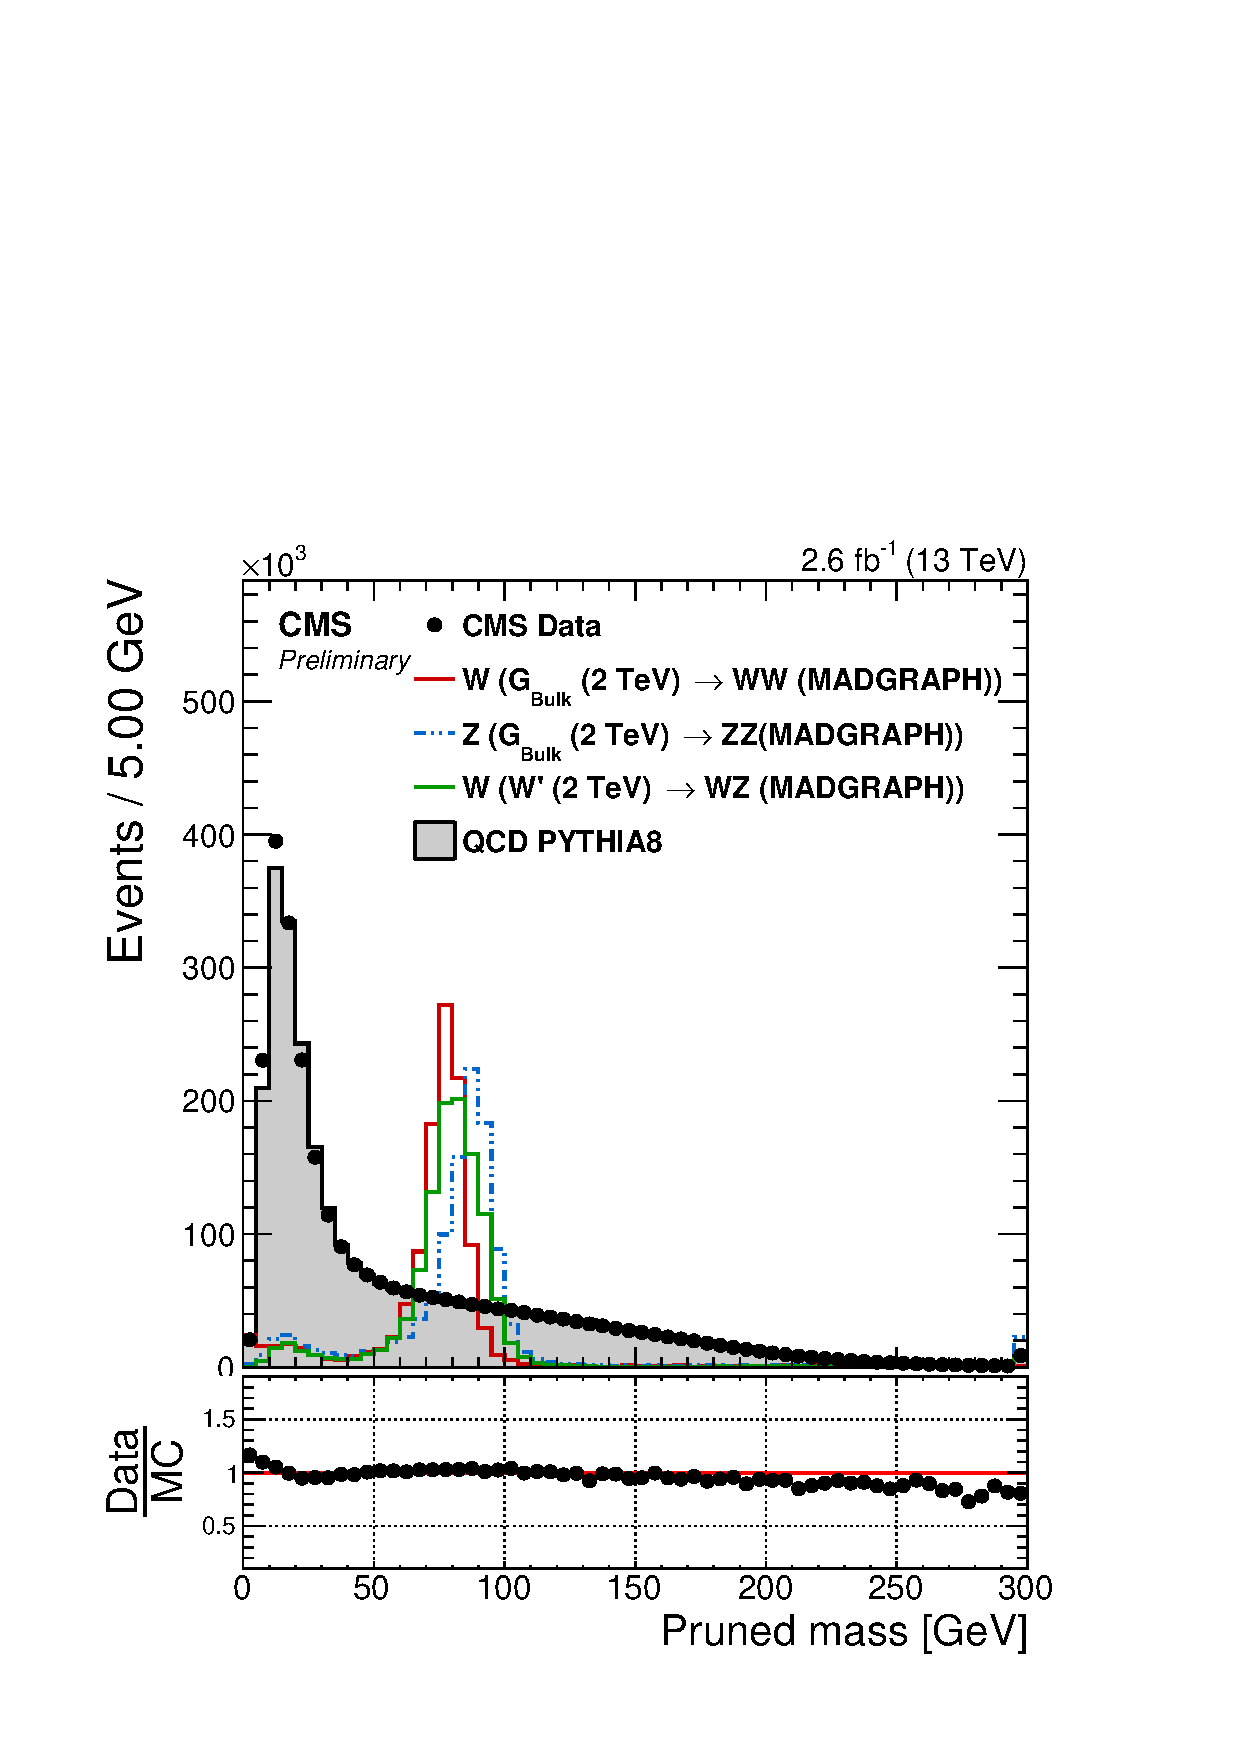
\includegraphics[width=0.4\textwidth]{figures/controlplots/silverjson/PrunedMass_WSignal.pdf}
% 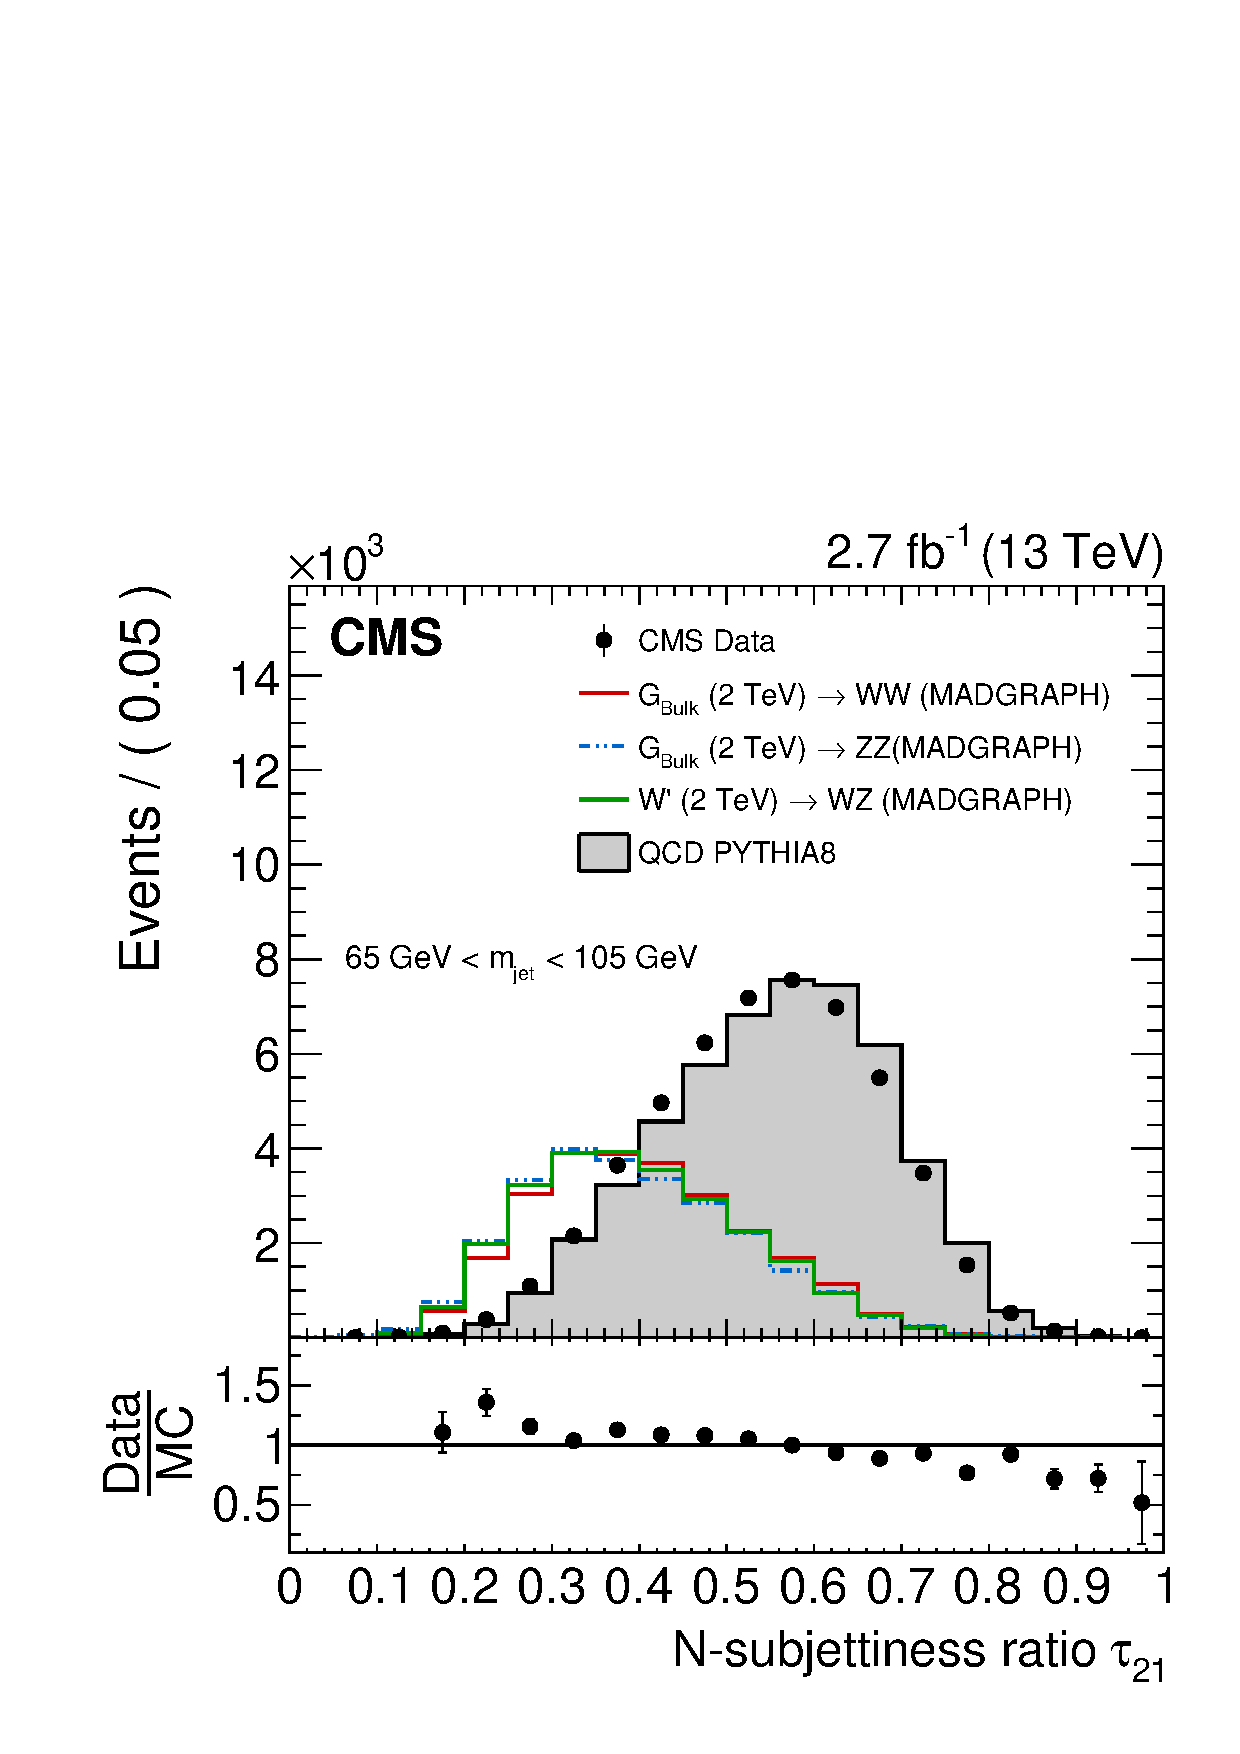
\includegraphics[width=0.4\textwidth]{figures/controlplots/silverjson/Tau21_punzi_WSignal.pdf}\\
% \caption{Pruned jet mass distribution (left) and n-subjettiness $\tau_{21}$ (right) distribution for data and simulated samples. Simulated samples are scaled to match the distribution in data. The $\tau_{21}$ distribution is shown for jets after a cut of $65 {\GeV} < M_{p} < 105 {\GeV}$ has been applied.}
% \label{fig:wtag}
% \end{figure}
%
% In order to enhance the analysis sensitivity, we further split the pruned jet mass window into a W and a Z boson window where the W window is defined as $65 {\GeV} < M_{p} < 85 {\GeV}$ and the Z boson window as $85 {\GeV} < M_{p} < 105 {\GeV}$.
% This allows us to make an estimate of how WW/ZZ/WZ or qW/qZ -like our signal is by counting events in each category. We for instance expect a higher signal yield in WZ category for a W’ decaying to a W and Z boson then for a Graviton decaying to WW or ZZ. All categories are combined in the end, leading to the same or better sensitivity than when using the whole pruned mass window. With the high-purity and low-purity categories as defined above for each mass window combination, this leaves us with ten different signal categories. They are as follows:
% \begin{itemize}
% \item High-purity double W/Z-tag, 3 mass categories: WW, ZZ and WZ
% \item Low-purity double W/Z-tag, 3 mass categories: WW, ZZ and WZ
% \item High-purity single W/Z-tag, 2 mass categories: qW and qZ
% \item Low-purity single W/Z-tag, 2 mass categories:q W and qZ
% \end{itemize}
% While the combination of the above listed categories define the main analysis strategy, we also perform two cross check analyses in parallel. An analysis without any selection on $\tau_{21}$ and categorizations in mass is intended to be a cross check analysis without sensitivity to the nature of the W/Z bosons, e.g. will also be sensitive to 3-prong particles with the same mass as the W and Z boson. We also provide plots analogous to the Run I result \cite{CMS-PAS-EXO-14-024}, where categorizations in $\tau_{21}$  was done, but no categorization in mass, thus the selection is labeled qV or VV.
% The tagging efficiency for different signals (RS and Bulk Graviton, W' and excited quarks q*) in the different signal categories as well as the signal efficiency in a region where no n-subjettiness cut is applied (NP), is shown in Figure~\ref{fig:sigeff}. The solid lines represent the tagging efficiency in the full mass window ($65 {\GeV} < M_{p} < 105 {\GeV}$) before splitting into mass categories. A lower signal efficiency the ZZ mass category is observed in all cases. This can be explained from the pruned jet mass distribution on the left in Figure~\ref{fig:wtag}, where a cut at 85 GeV leaves a large fraction of the Z peak in the W mass window. As the main benchmark models under consideration preferably decays to W bosons (in the Bulk Graviton model the branching ratio BR($G_{Bulk}$ $\rightarrow$ \PW\PW) = 2* BR($G_{Bulk}$$\rightarrow$ ZZ), and in the HVT model W'/Z' $\rightarrow$ WZ/WW (but not ZZ) ), a high tagging efficiency for the W boson is preferred. In the limit-setting procedure all the categories are combined and the overall signal efficiency is conserved. For the combined mass-categories (solid line) the signal efficiency is between 16 and 23 \% in the double-tag categories, and between 20 and 34 \% in the single-V tag categories. Figure~\ref{fig:bkgeff} shows the corresponding background mistagging efficiency in all channels. The mistagging rate in the double-V tag categories is below 1 \% in the high-purity category. A smooth background is expected from simulation in all cases, thus we expect to be able to describe the background with a smooth fit function.
%
% \begin{figure}[htb]
% \centering
%
% 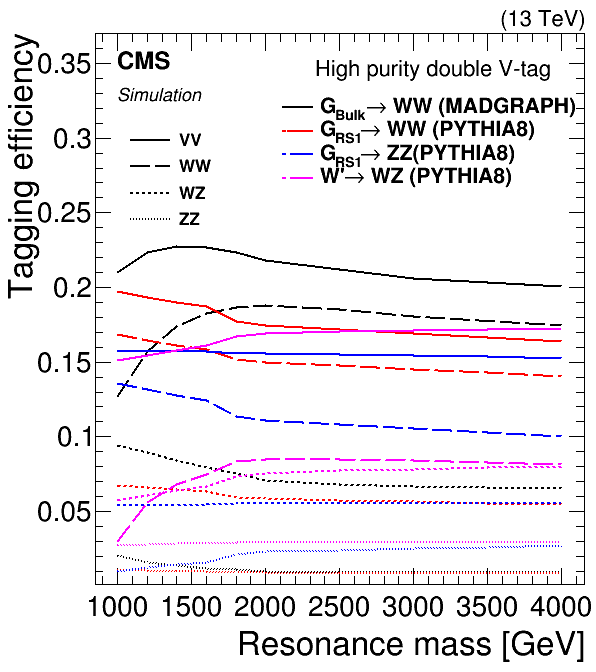
\includegraphics[width=0.4\textwidth]{figures/HP_VV_SigEff.png}
% 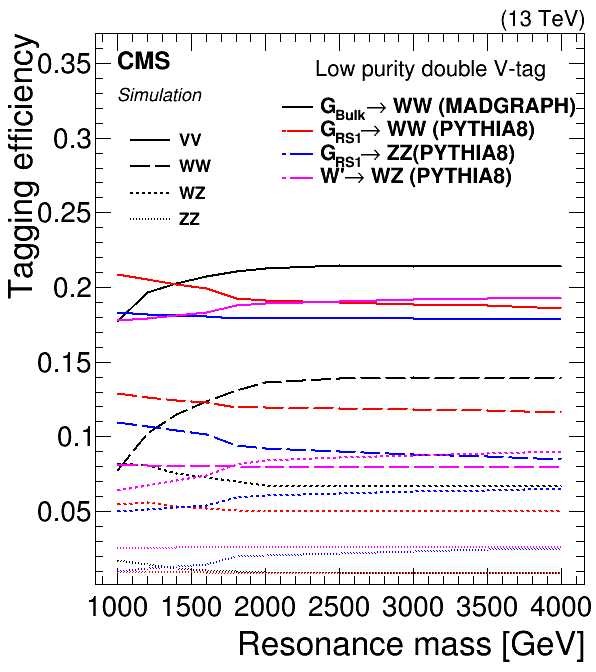
\includegraphics[width=0.4\textwidth]{figures/LP_VV_SigEff.png}\\
% 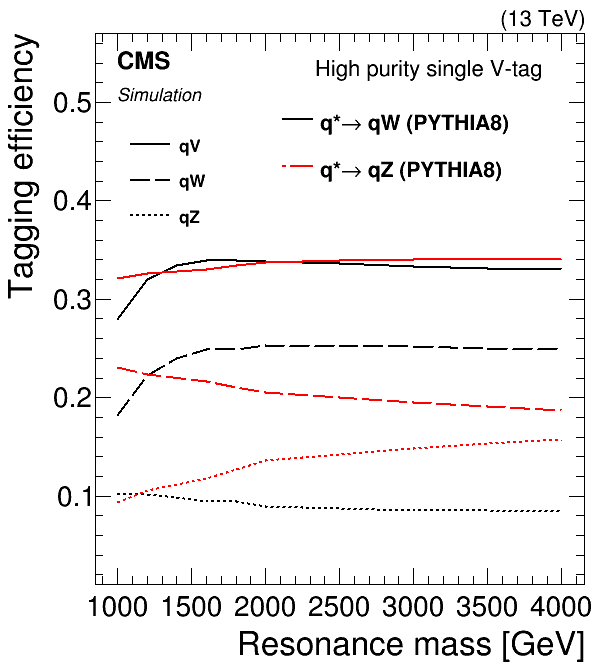
\includegraphics[width=0.4\textwidth]{figures/HP_qV_SigEff.png}
% 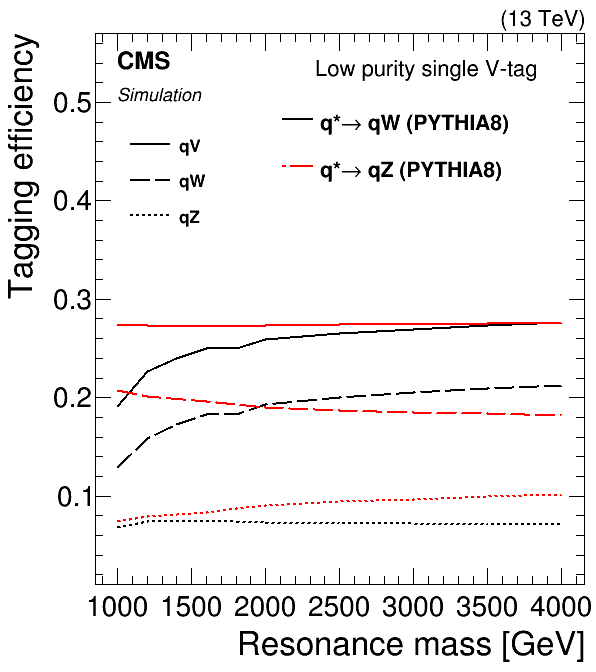
\includegraphics[width=0.4\textwidth]{figures/LP_qV_SigEff.png}\\
% 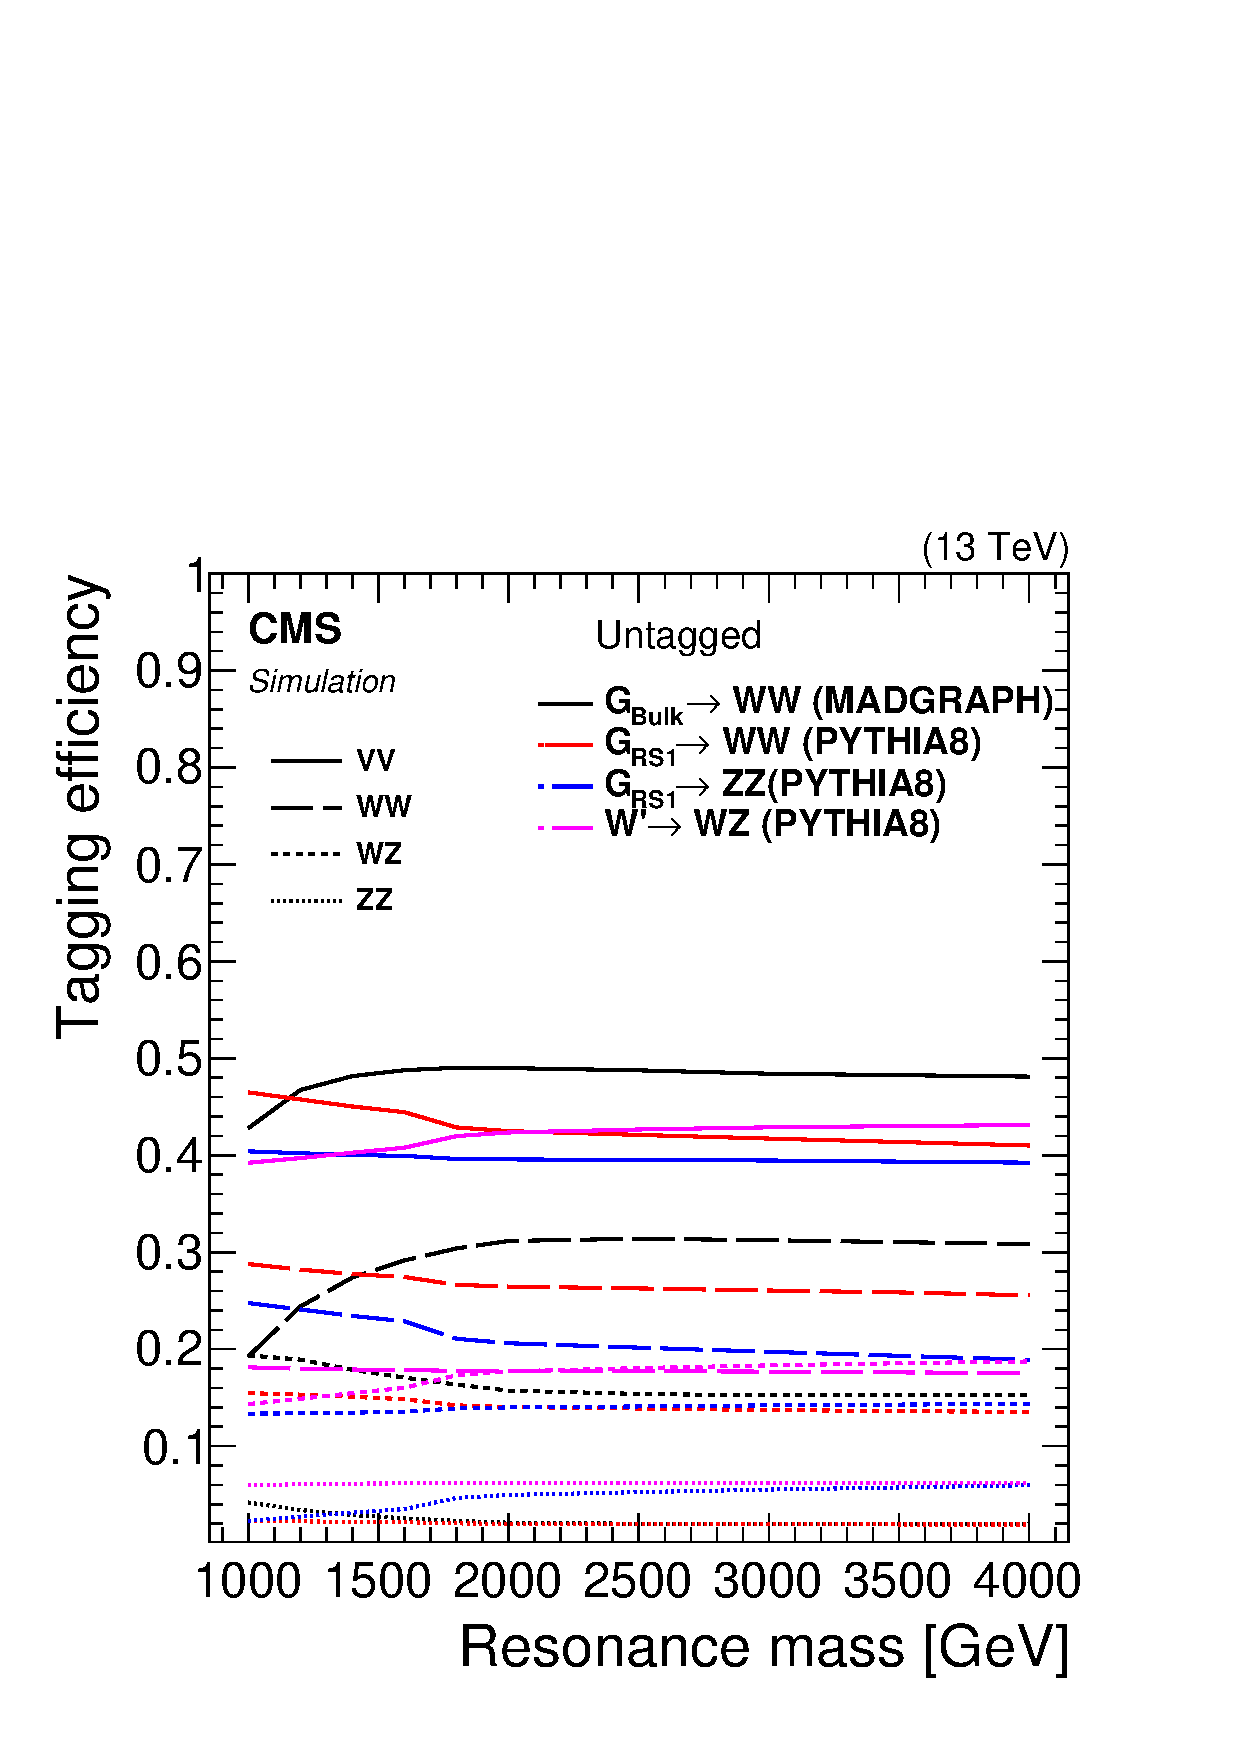
\includegraphics[width=0.4\textwidth]{figures/NP_VV_SigEff.pdf}
% 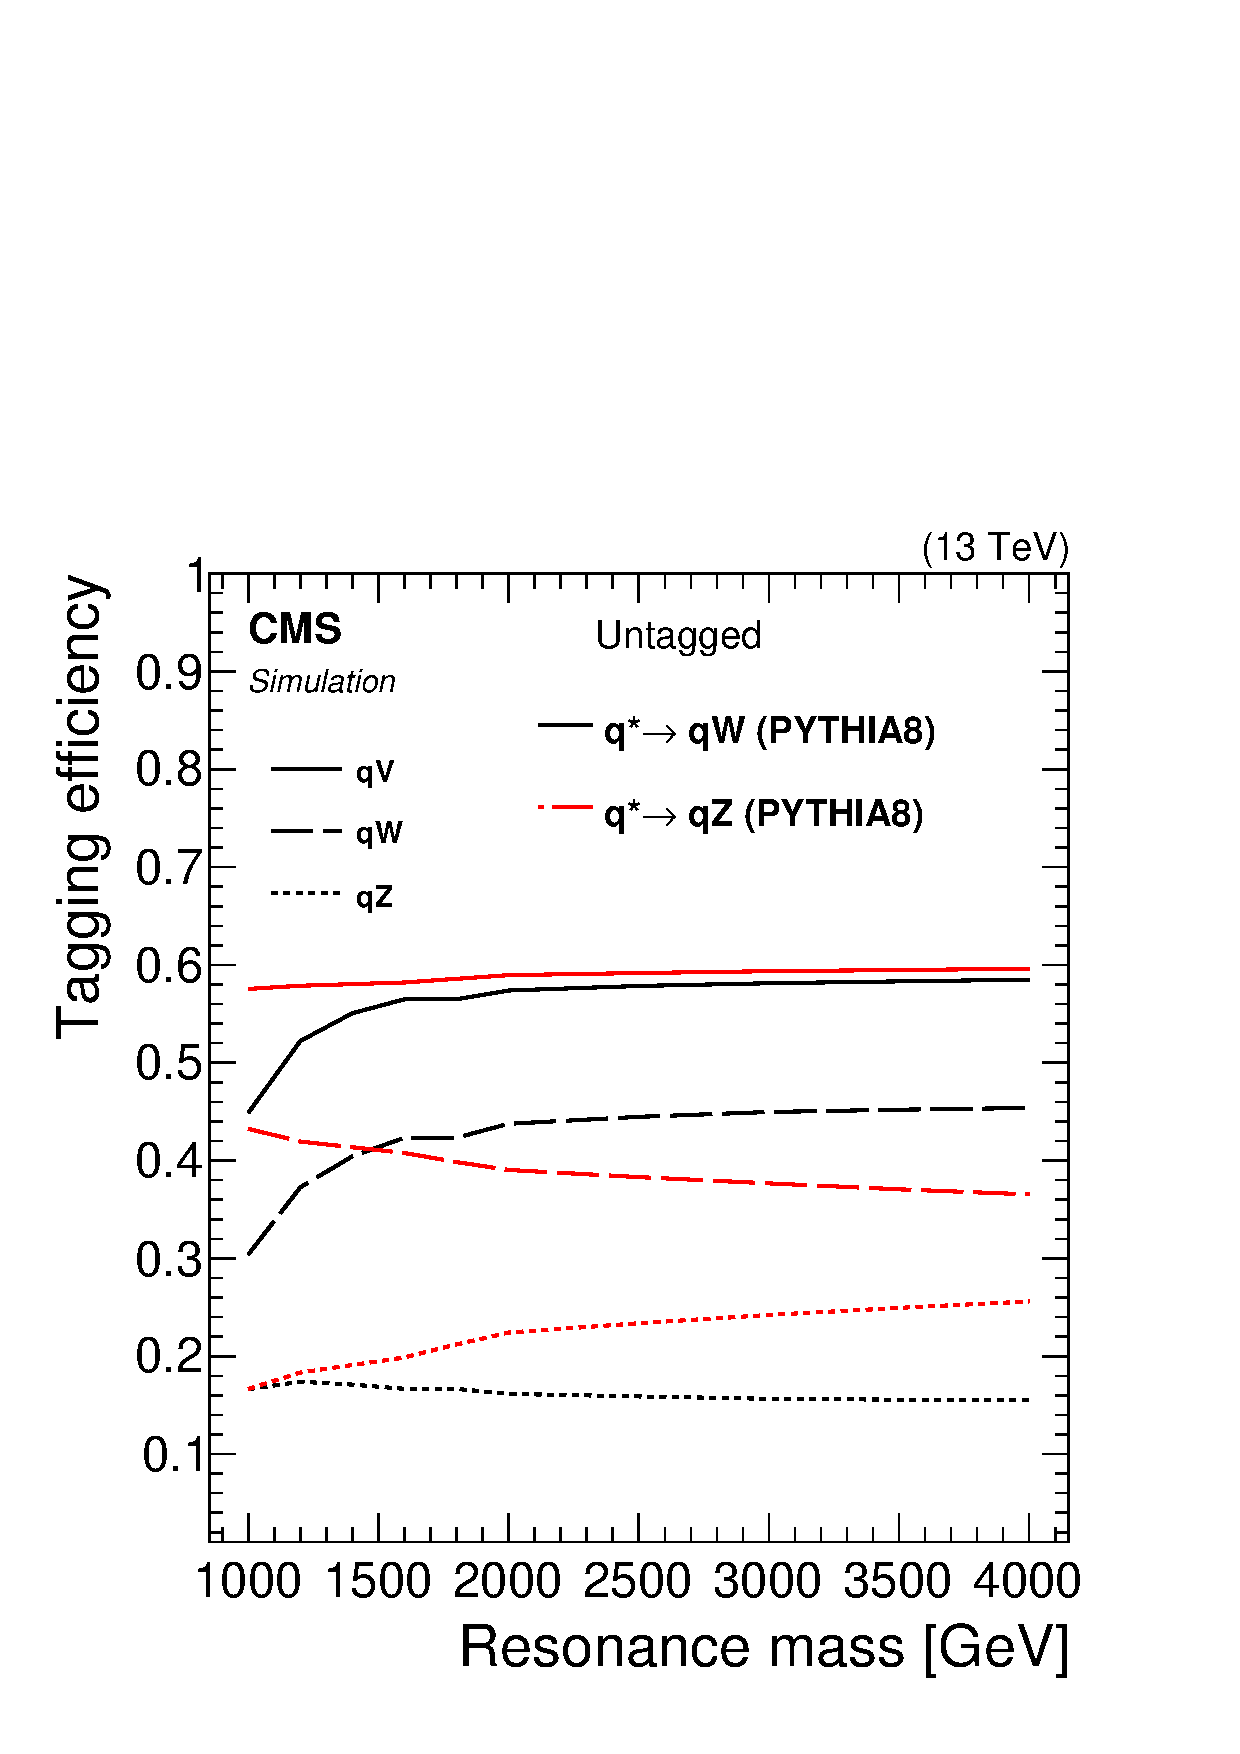
\includegraphics[width=0.4\textwidth]{figures/NP_qV_SigEff.pdf}\\
% \caption{Tagging efficiency in the different pruned mass categories in the high-purity double-V tag category (top left),in the low-purity double-V tag category (top right), in the high-purity single-V tag category (middle left), the low-purity single-V tag category (middle right), and in a region with no n-subjettiness cut applied for the double-V tag (left) and single-V tag (right) categories.}
% \label{fig:sigeff}
% \end{figure}
%
%
% \begin{figure}[htb]
% \centering
% 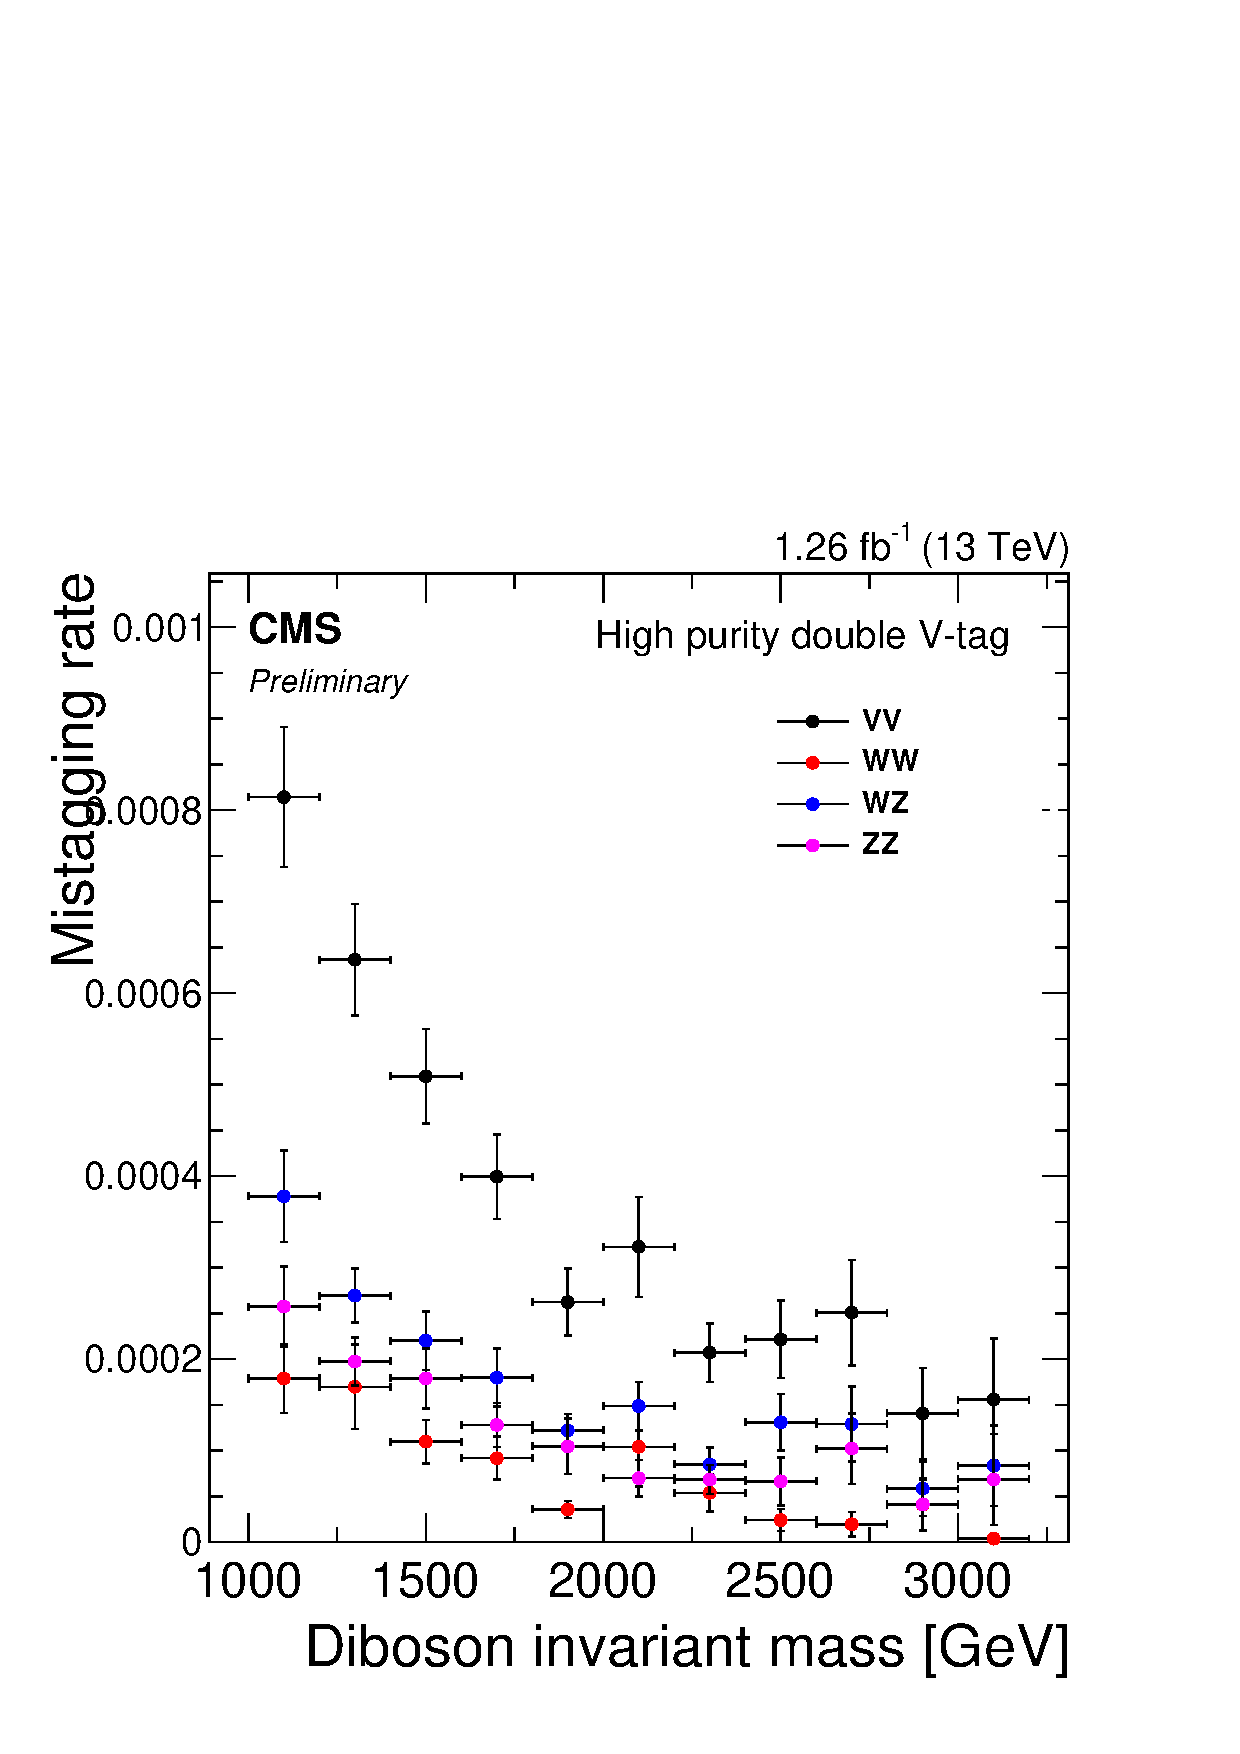
\includegraphics[width=0.4\textwidth]{figures/QCD_HP_VV_MistaggingRateEff.pdf}
% 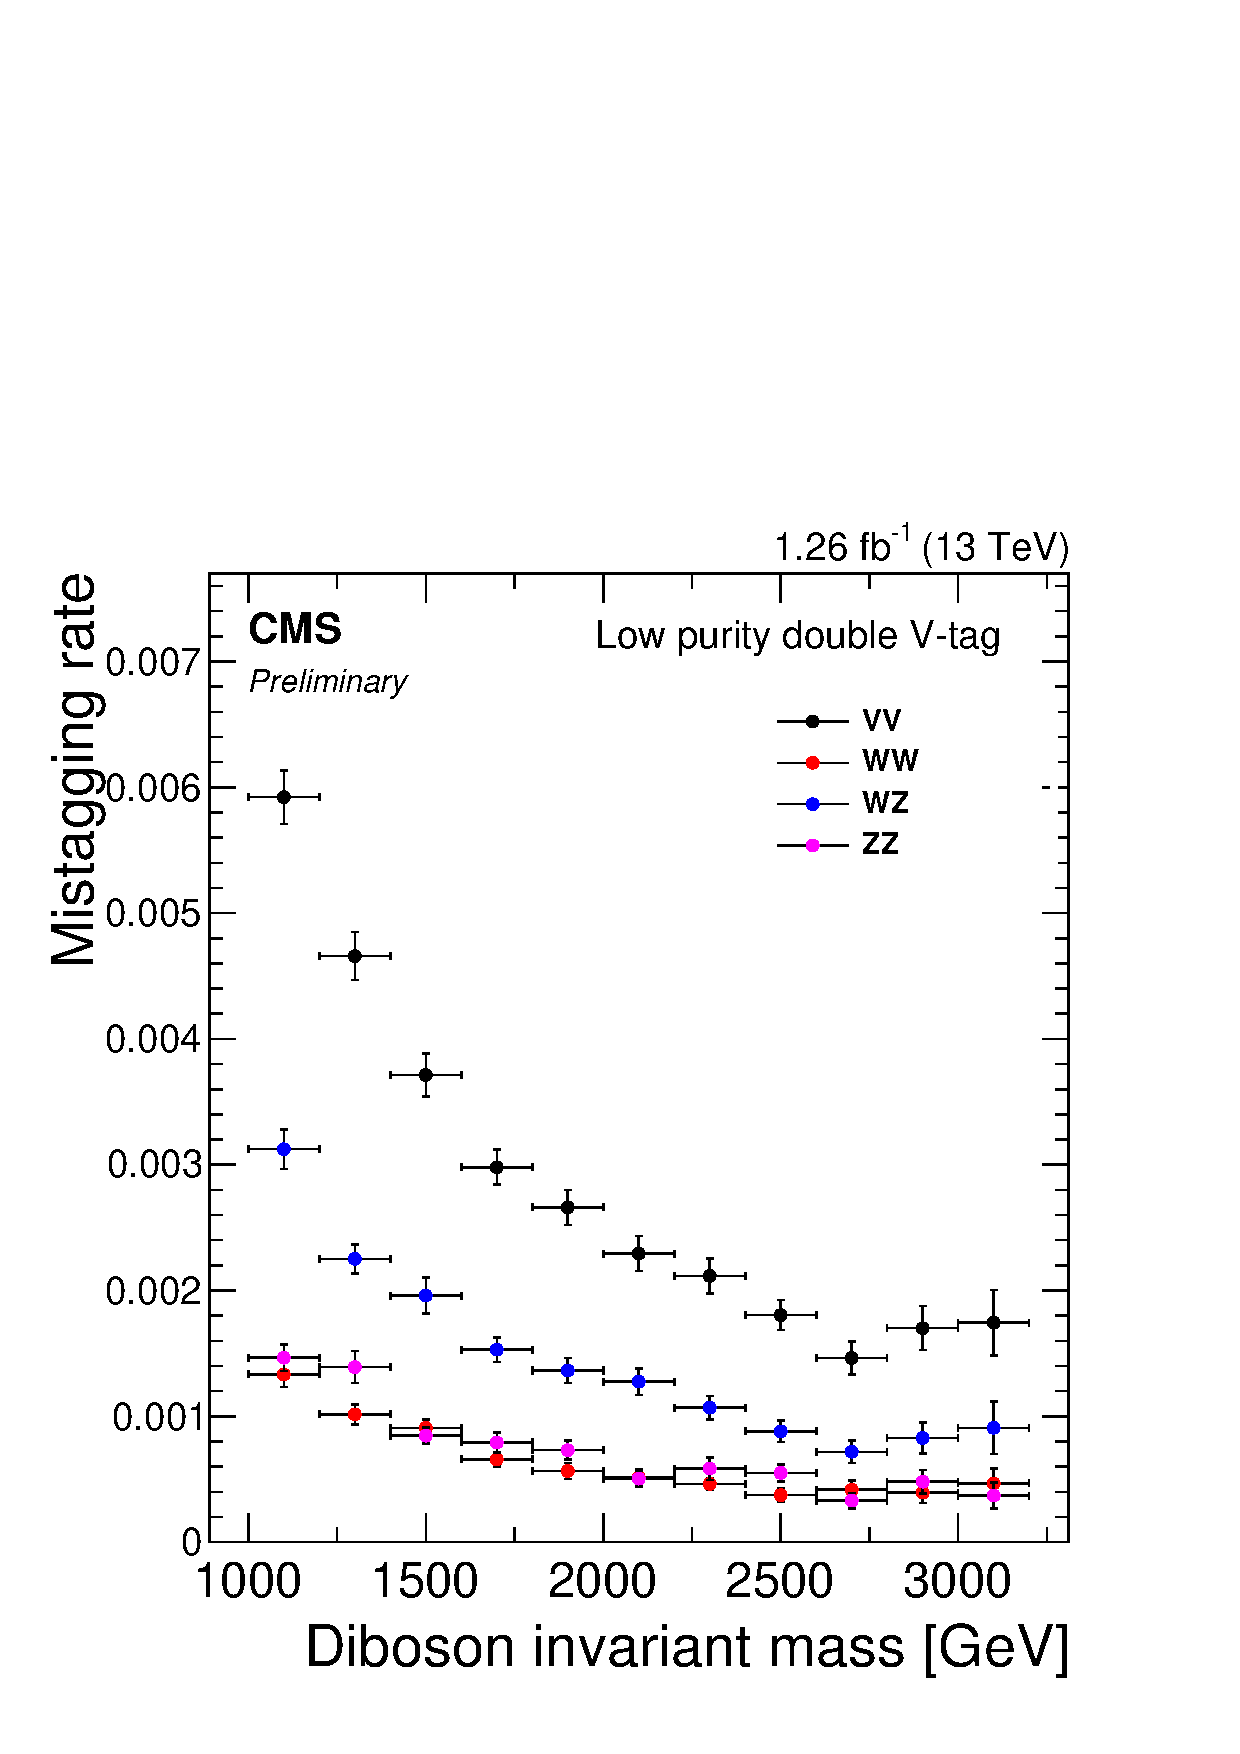
\includegraphics[width=0.4\textwidth]{figures/QCD_LP_VV_MistaggingRateEff.pdf}
% 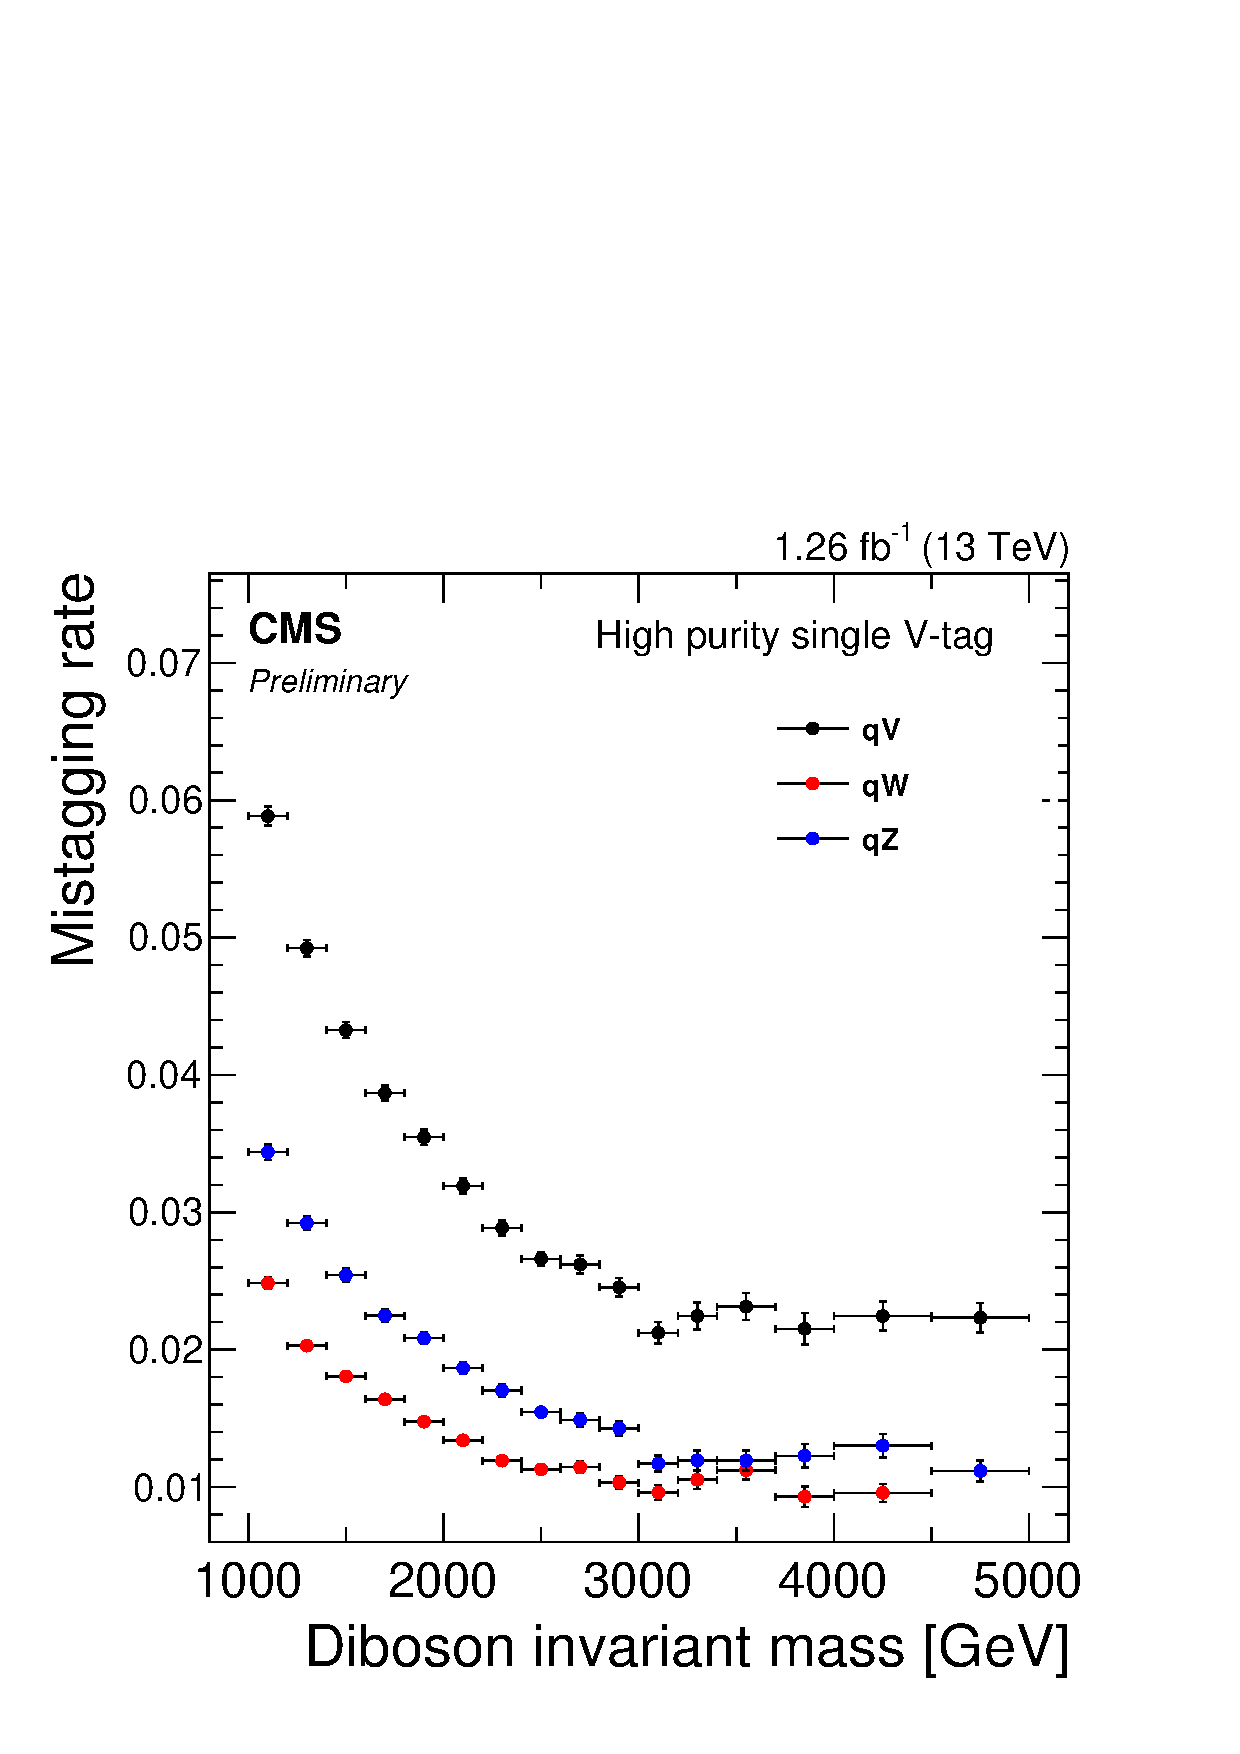
\includegraphics[width=0.4\textwidth]{figures/QCD_HP_qV_MistaggingRateEff.pdf}
% 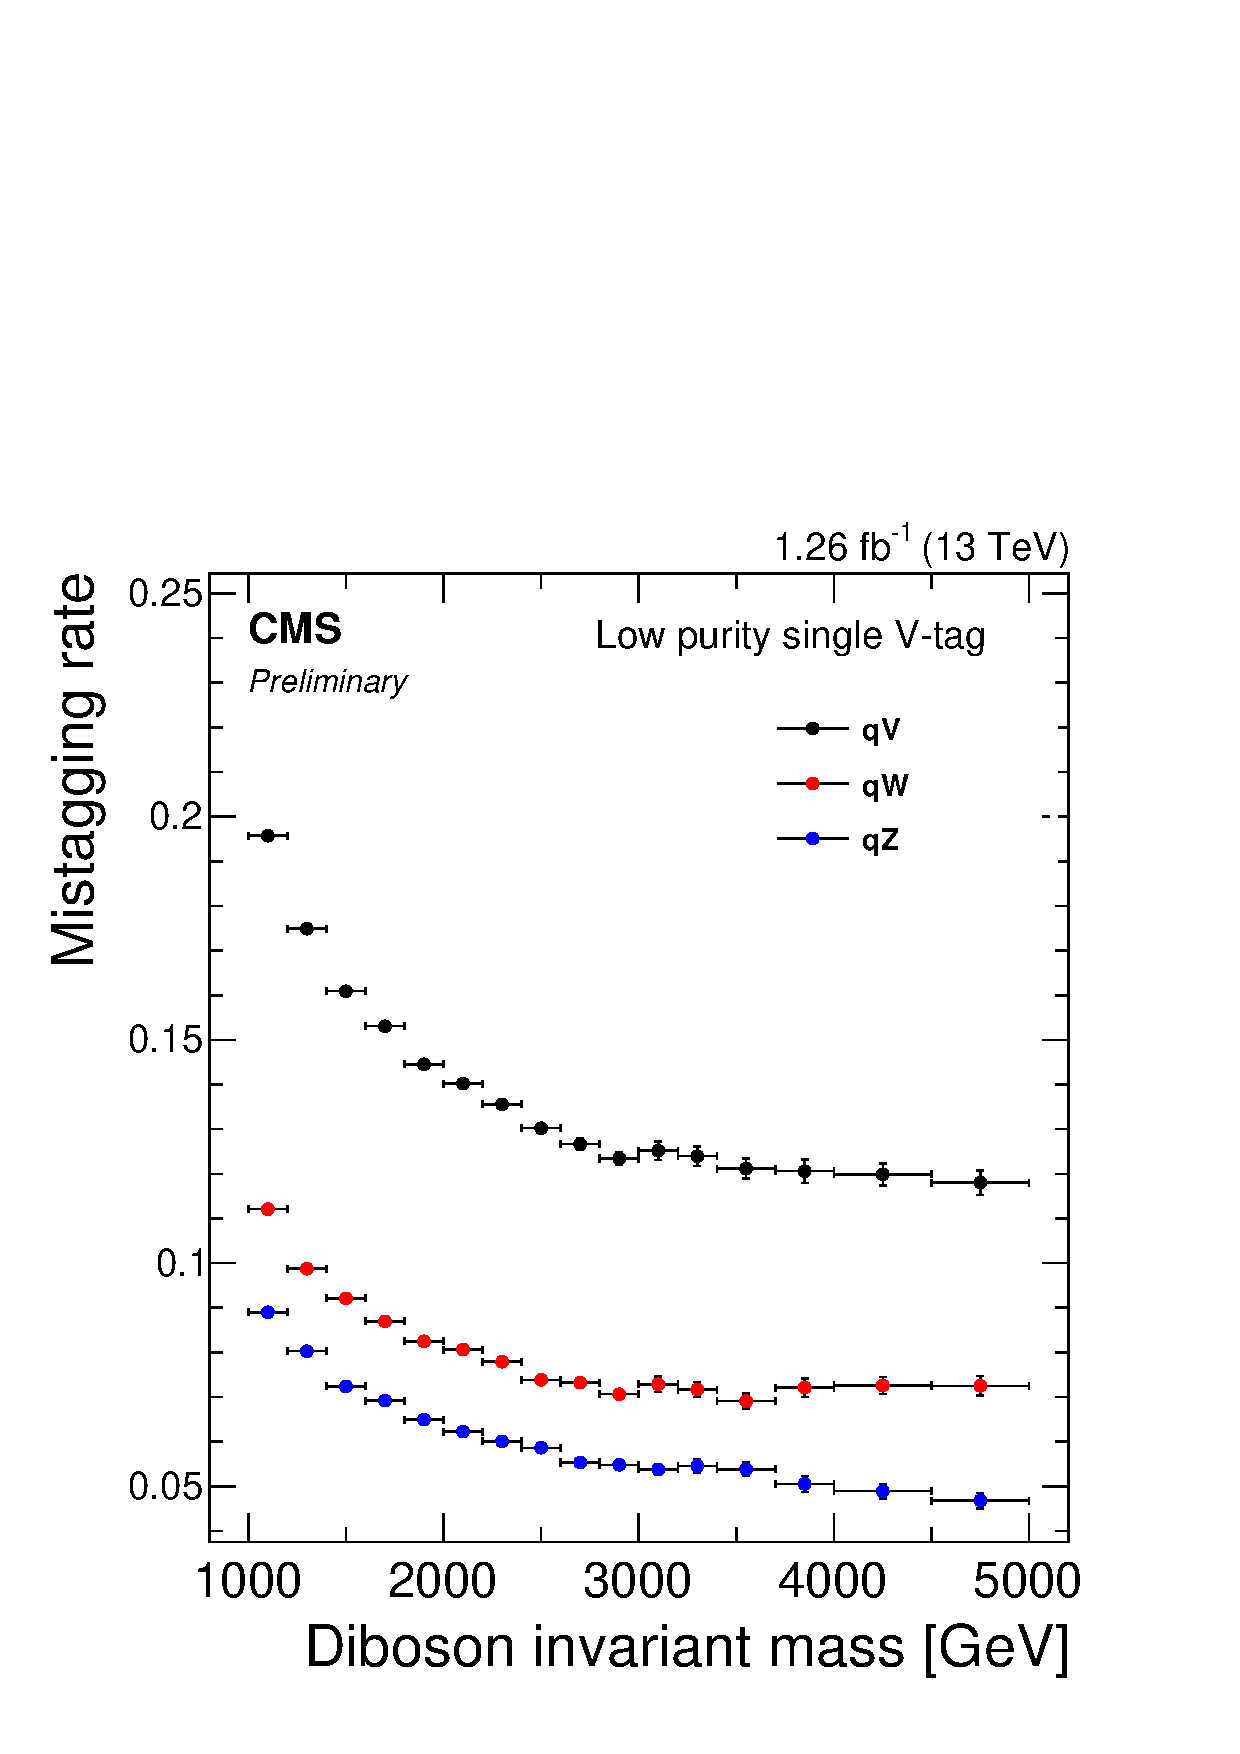
\includegraphics[width=0.4\textwidth]{figures/QCD_LP_qV_MistaggingRateEff.pdf}
% 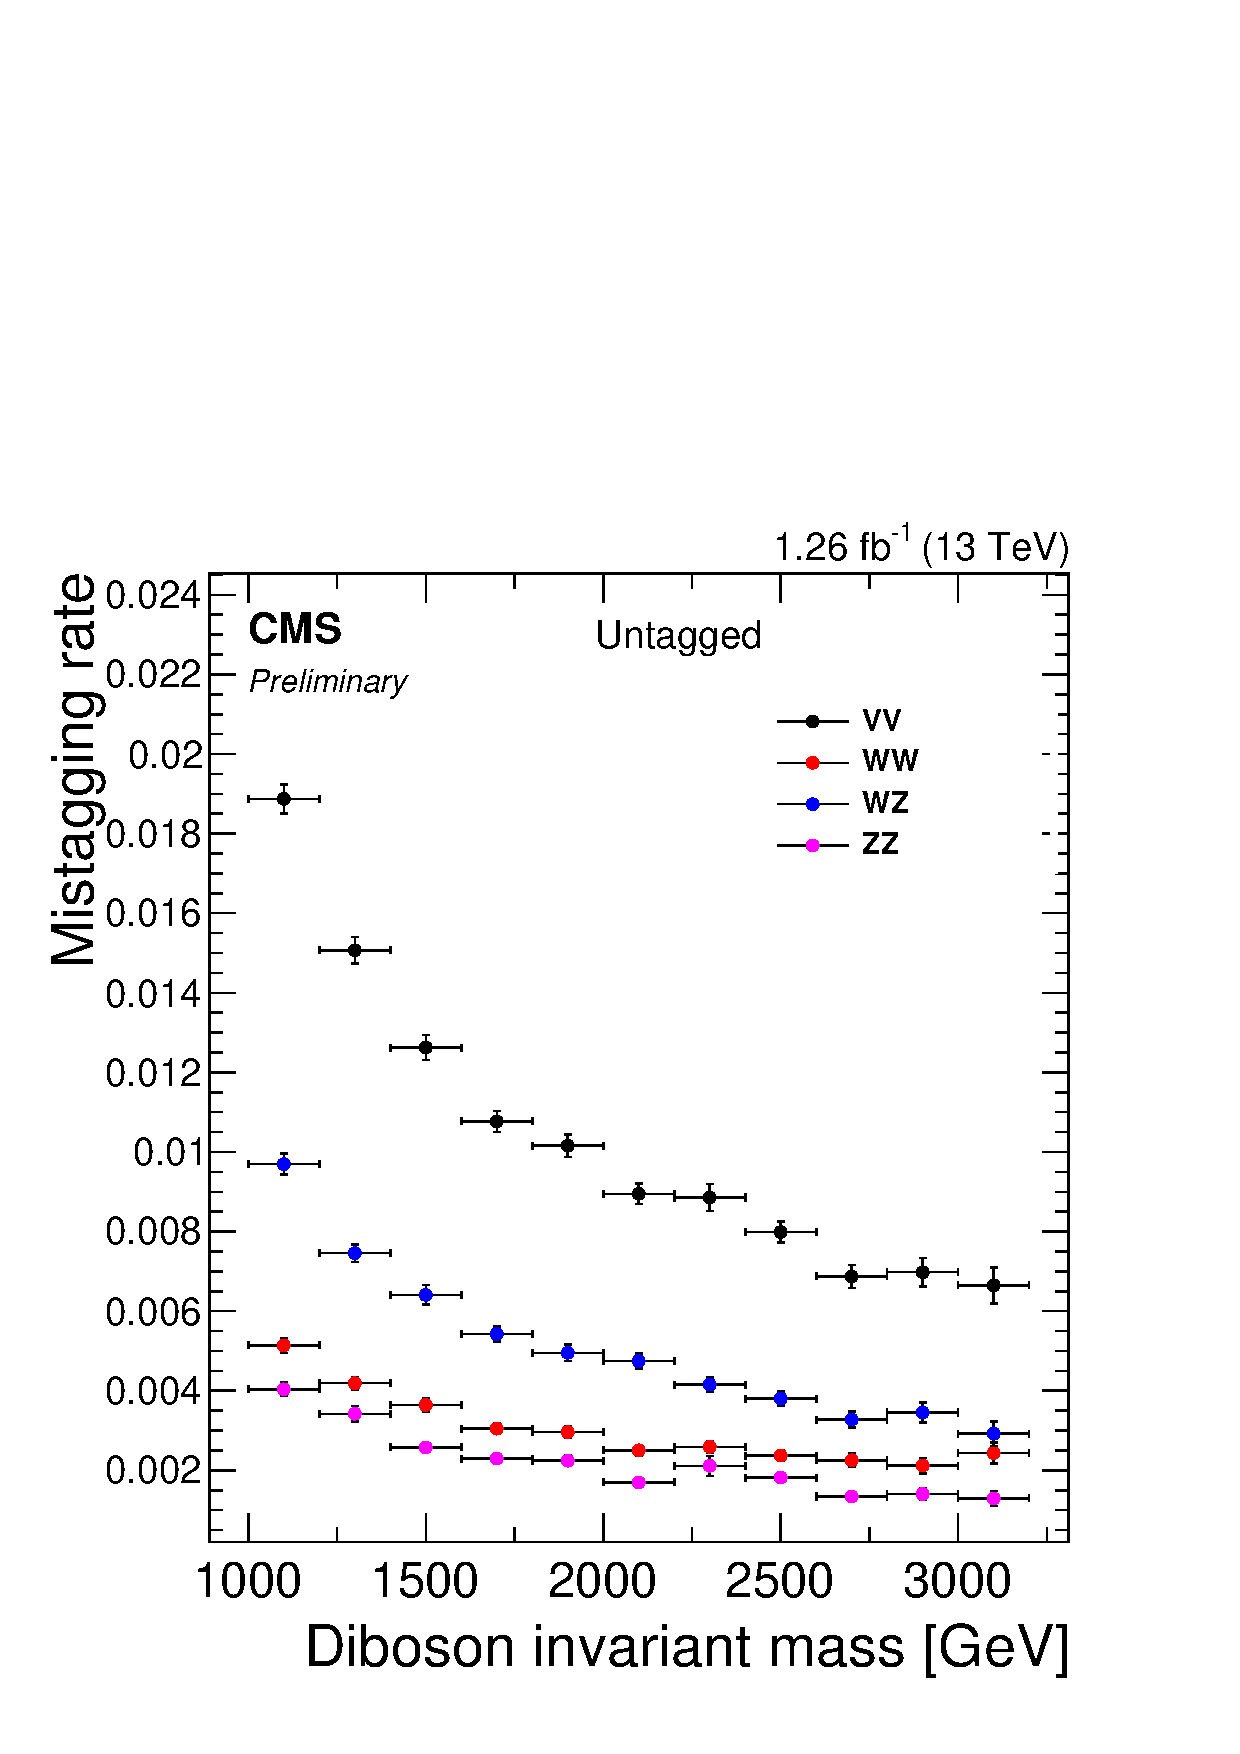
\includegraphics[width=0.4\textwidth]{figures/QCD_NP_VV_MistaggingRateEff.pdf}
% 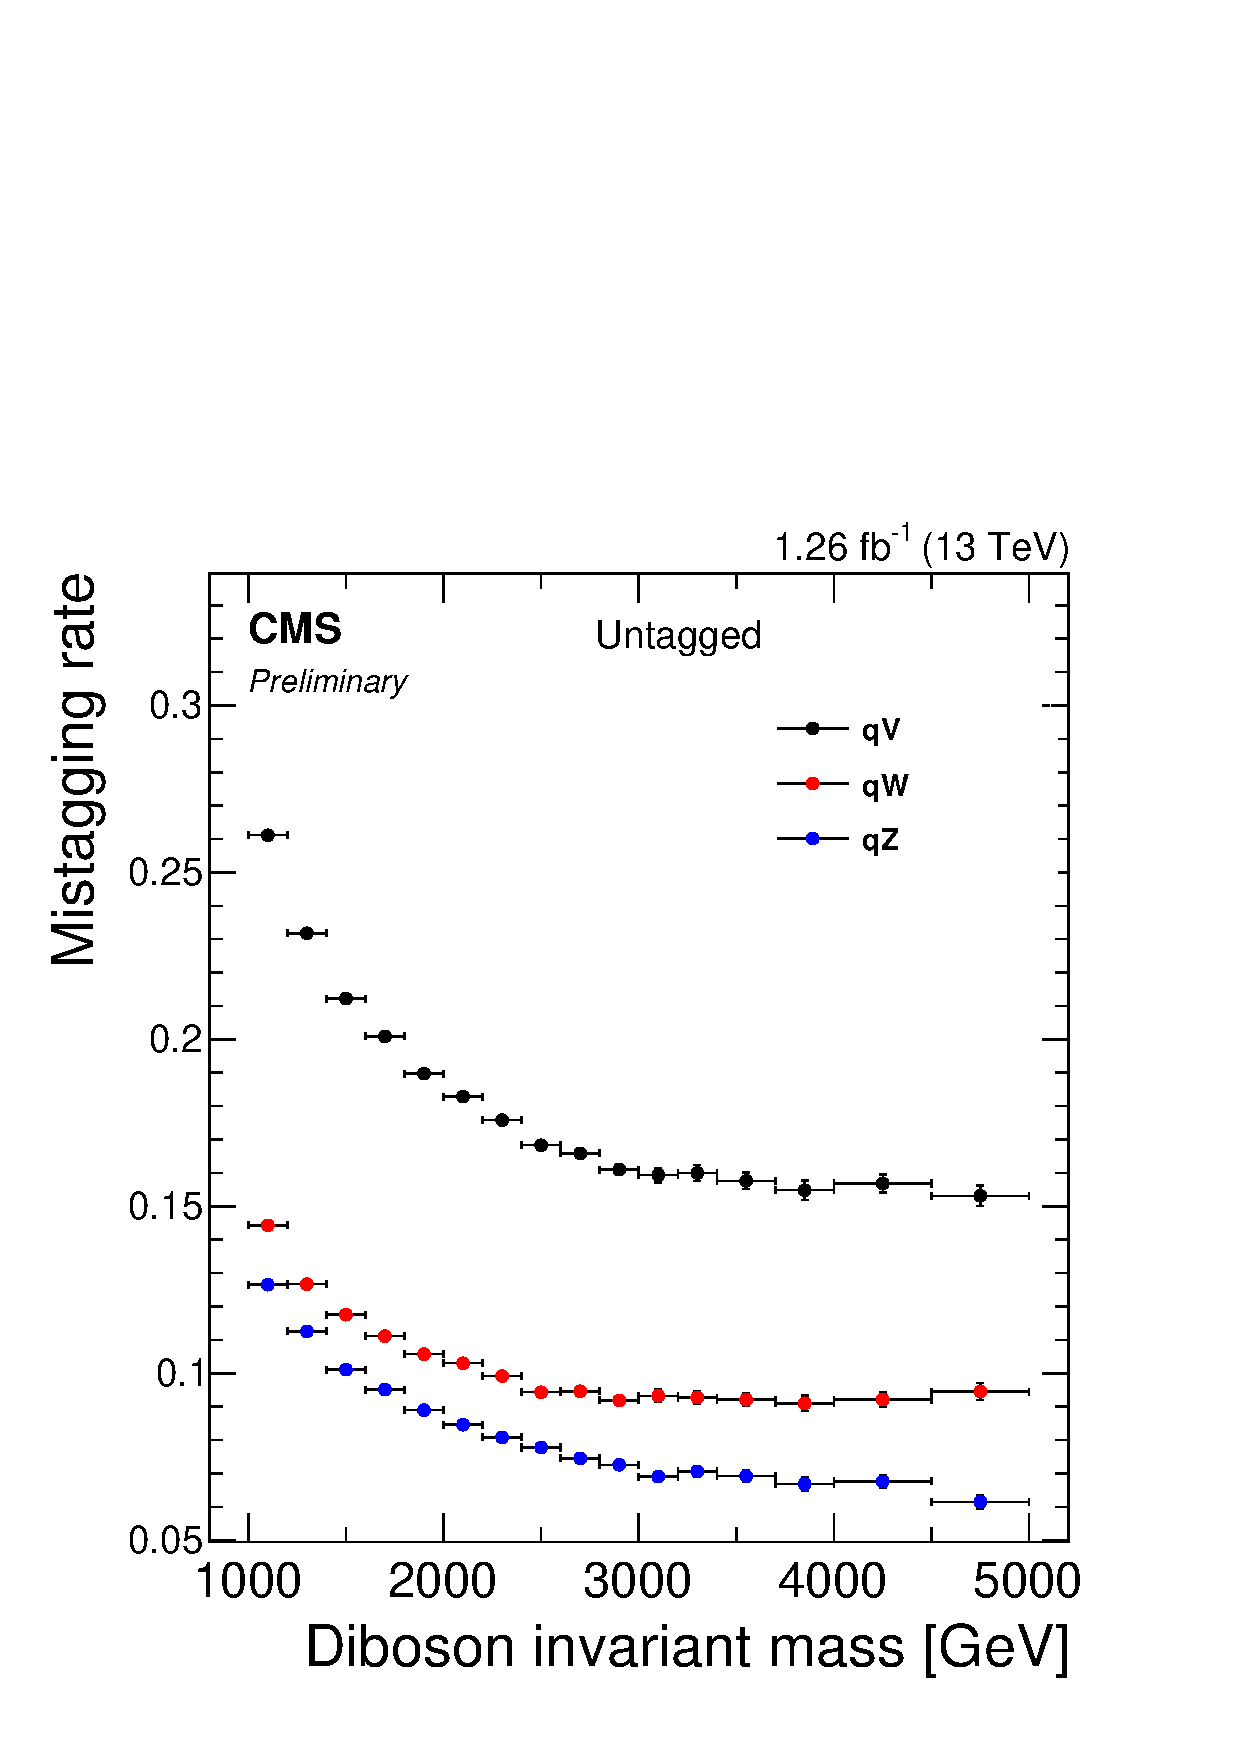
\includegraphics[width=0.4\textwidth]{figures/QCD_NP_qV_MistaggingRateEff.pdf}
% \caption{Mistagging rate in the different pruned mass categories in the high-purity double-V tag category (top left),in the low-purity double-V tag category (top right), in the high-purity single-V tag category (middle left), the low-purity single-V tag category (middle right), and in a region with no n-subjettiness cut applied for the double-V tag (left) and single-V tag (right) categories.}
% \label{fig:bkgeff}
% \end{figure}



\subsection{Background modeling}
\label{sec:searchI:bkg}


